\PassOptionsToPackage{dvipsnames}{xcolor} % Added for new colors.
% Fixing: Too many math alphabets used in version normal
\newcommand\hmmax{0}
\newcommand\bmmax{0}
\documentclass[acmsmall]{acmart}
%%
%% \BibTeX command to typeset BibTeX logo in the docs
\AtBeginDocument{%
  \providecommand\BibTeX{{%
    Bib\TeX}}}

%% Rights management information.  This information is sent to you
%% when you complete the rights form.  These commands have SAMPLE
%% values in them; it is your responsibility as an author to replace
%% the commands and values with those provided to you when you
%% complete the rights form.
\setcopyright{acmlicensed}
\copyrightyear{2018}
\acmYear{2018}
\acmDOI{XXXXXXX.XXXXXXX}

%%
%% These commands are for a JOURNAL article.
\acmJournal{JACM}
\acmVolume{37}
\acmNumber{4}
\acmArticle{111}
\acmMonth{8}

%%
%% Submission ID.
%% Use this when submitting an article to a sponsored event. You'll
%% receive a unique submission ID from the organizers
%% of the event, and this ID should be used as the parameter to this command.
%%\acmSubmissionID{123-A56-BU3}

%%
%% For managing citations, it is recommended to use bibliography
%% files in BibTeX format.
%%
%% You can then either use BibTeX with the ACM-Reference-Format style,
%% or BibLaTeX with the acmnumeric or acmauthoryear sytles, that include
%% support for advanced citation of software artefact from the
%% biblatex-software package, also separately available on CTAN.
%%
%% Look at the sample-*-biblatex.tex files for templates showcasing
%% the biblatex styles.
%%

%%
%% The majority of ACM publications use numbered citations and
%% references.  The command \citestyle{authoryear} switches to the
%% "author year" style.
%%
%% If you are preparing content for an event
%% sponsored by ACM SIGGRAPH, you must use the "author year" style of
%% citations and references.
%% Uncommenting
%% the next command will enable that style.
%%\citestyle{acmauthoryear}

\usepackage[T1]{fontenc}
\usepackage[scaled=.83]{beramono}

\usepackage[colorinlistoftodos]{todonotes}
\usepackage[inference]{semantic}
\usepackage[dvipsnames]{xcolor}
\usepackage[switch]{lineno}
\usepackage{halloweenmath}
\usepackage{fontawesome5}
\usepackage{listofitems}
\usepackage{breakcites}
\usepackage{glossaries}
\usepackage{hyperref}
\usepackage{cleveref}
\usepackage{stmaryrd}
\usepackage{marvosym}
\usepackage{listings}
\usepackage{amsmath}
\usepackage{nameref}
\usepackage{amsthm}
\usepackage{xspace}
\usepackage{xfrac}
\usepackage{tikz}
\usepackage{soul}
\usepackage{bm}
\usepackage{paralist}

\hypersetup{
    colorlinks,
    linkcolor={red!50!black},
    citecolor={blue!50!black},
    urlcolor={blue!80!black}
}
%\renewcommand\UrlFont{\color{blue}\rmfamily}
%\newcommand{\url}[1]{\lstinline{#1}}

\setul{0.95ex}{0.3ex}


\usetikzlibrary{calc,decorations.pathmorphing,shapes,positioning}
\newcounter{sarrow}
\newcommand\xrsquigarrow[1]{%
\stepcounter{sarrow}%
\mathrel{\begin{tikzpicture}[baseline= {( $ (current bounding box.south) + (0,-0.5ex) $ )}]
\node[inner sep=.5ex] (\thesarrow) {$\scriptstyle #1$};
\path[draw,<-,decorate,
  decoration={zigzag,amplitude=0.7pt,segment length=1.2mm,pre=lineto,pre length=4pt}]
    (\thesarrow.south east) -- (\thesarrow.south west);
\end{tikzpicture}}%
}
\makeatletter
\newcommand{\xRightarrow}[2][]{\ext@arrow 0359\Rightarrowfill@{#1}{#2}}
\makeatother

\newcommand{\thmref}[1]{\cref{#1}~(\nameref{#1})}
\newcommand{\Thmref}[1]{\Cref{#1}~(\nameref{#1})}

%%%%
% TODO macros
\newcommand{\MK}[1]{\todo[color=orange!30]{TODO: #1}}
\newcommand{\MKin}[1]{\todo[color=orange!30,inline]{TODO: #1}}
\newcommand{\MP}[1]{\todo[color=blue!30]{TODO: #1}}
\newcommand{\MPin}[1]{\todo[color=blue!30,inline]{TODO: #1}}
\newcommand{\hltt}[1]{\begin{center}\fbox{\color{green}\large{#1}}\end{center}}

% Approx
\newcommand{\pages}[1]{}%\xspace\todo{\textbf{($\sim$#1 pages)}\xspace}}

%%%%
% Colors
\newcommand{\neutcol}[0]{black}
\newcommand{\stlccol}[0]{RoyalBlue}
\newcommand{\irccol}[0]{Apricot}
\newcommand{\ulccol}[0]{RedOrange}
\newcommand{\objcol}[0]{Emerald} %CarnationPink}
\newcommand{\commoncol}[0]{black}

\newcommand{\col}[2]{\ensuremath{{\color{#1}{#2}}}}

\newcommand{\com}[1]{\ensuremath\mathit{\col{\neutcol}{#1}}}
\newcommand{\src}[1]{\ensuremath\mathsf{\col{\stlccol}{#1}}}
\newcommand{\irl}[1]{\ensuremath\mathit{\col{\irccol}{#1}}}
\newcommand{\trg}[1]{\ensuremath\mathbf{\col{\ulccol}{#1}}}
\newcommand{\obj}[1]{\ensuremath\mathtt{\col{\objcol}{#1}}}

%%%%
% Text Decorations
\newcommand\BrText[2]{%
  \par\smallskip
   \noindent\makebox[\textwidth][r]{$\text{\scriptsize #1}\left\{
    \begin{minipage}{\textwidth}
    #2
    \end{minipage}
  \right.\nulldelimiterspace=0pt$}\par\smallskip
}
\newcommand{\mi}[1]{\ensuremath{\mathit{#1}}}
\newcommand{\mr}[1]{\ensuremath{\mathrm{#1}}}
\newcommand{\mt}[1]{\ensuremath{\texttt{#1}}}
\newcommand{\mtt}[1]{\ensuremath{\mathtt{#1}}}
\newcommand{\mf}[1]{\ensuremath{\mathbf{#1}}}
\newcommand{\mk}[1]{\ensuremath{\mathfrak{#1}}}
\newcommand{\mc}[1]{\ensuremath{\mathcal{#1}}}
\newcommand{\ms}[1]{\ensuremath{\mathsf{#1}}}
\newcommand{\mb}[1]{\ensuremath{\mathbb{#1}}}
\newcommand{\msc}[1]{\ensuremath{\mathscr{#1}}}

\newcommand{\bul}[1]{{\setulcolor{RoyalBlue}\ul{#1}}}
\newcommand{\rul}[1]{{\setulcolor{RedOrange}\ul{#1}}}
\newcommand{\iul}[1]{{\setulcolor{Apricot}\ul{#1}}}
\newcommand{\oul}[1]{{\setulcolor{Emerald}\ul{#1}}}
\newcommand{\pul}[1]{{\setulcolor{CarnationPink}\ul{#1}}}

\newcommand{\lock}{\ensuremath\text{\scriptsize\faIcon{lock}}}
\newcommand{\unlock}{\ensuremath\text{\scriptsize\faIcon{lock-open}}}

\newcommand{\tup}[2]{\ensuremath (#1 %
  \readlist\myterms{#2}%
  \foreachitem\x\in\myterms{;\x}%
  )%
}

\newcommand{\isdef}[0]{\ensuremath{\mathrel{\overset{\makebox[0pt]{\mbox{\normalfont\tiny\sffamily def}}}{=}}}}

%%%%
% List of contributions
\newcounter{contrib}
\newcommand{\contribnum}[0]{\stepcounter{contrib}{\arabic{contrib}}.~}
\newcommand{\contribution}[1]{\smallskip\noindent\textbf{{#1.}\xspace}}

%%%%
% A symbol for Coq-verified theorems.
\newcommand{\BareCoqSymbol}{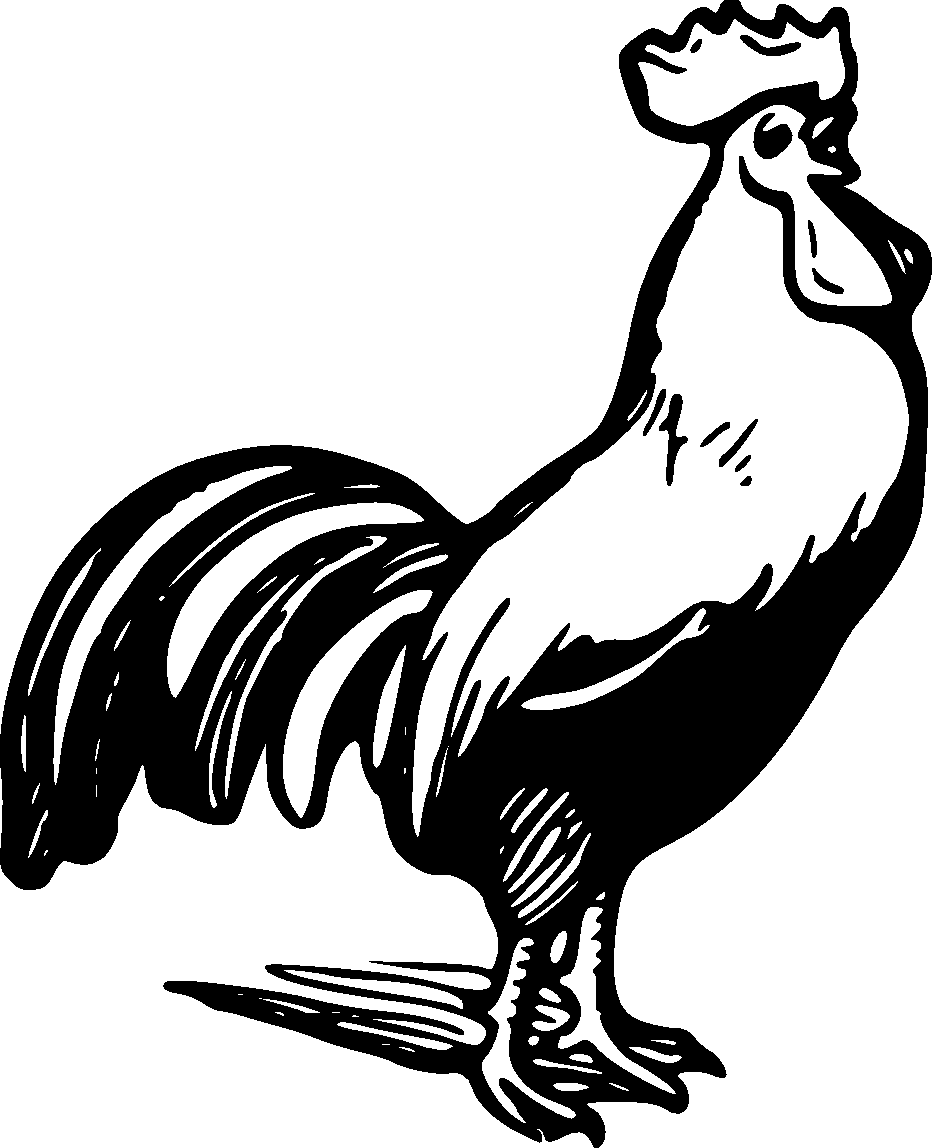
\includegraphics[height=0.9em]{coq.pdf}}
\newcommand{\CoqSymbol}{\raisebox{-.2ex}{\BareCoqSymbol\,}}
\newcommand{\Coqed}{\hfill\CoqSymbol}

\newcommand{\BareInvCoqSymbol}{
\includegraphics[height=0.9em]{inv_coq.png}}
\newcommand{\InvCoqSymbol}{\raisebox{-.2ex}{\BareInvCoqSymbol\,}}

%%%%
% Typerules
\newcommand{\textgraybox}[1]{\boxed{#1}}
\newdimen\zzfontsz
\newcommand{\fontsz}[2]{\zzfontsz=#1%
{\fontsize{\zzfontsz}{1.2\zzfontsz}\selectfont{#2}}}
\newcommand{\mathsz}[2]{\text{\fontsz{#1}{$#2$}}}
\newcommand{\instsymColon}{%
     \raisebox{-0.09ex}{\text{\normalfont{:}}}}
\newcommand{\judgboxfontsize}[1]{%
        \mathsz{11pt}{#1}%
}
\newcommand{\judgbox}[2]{%
      {\raggedright \textgraybox{\ensuremath{\judgboxfontsize{#1}}}\!%
        \fontsz{9pt}{\begin{tabular}[c]{l} #2 \end{tabular}} %
}}
\newcounter{typerule}
\crefname{typerule}{rule}{rules}

\newcommand{\typeruleInt}[5]{%
	\def\thetyperule{#1}%
	\refstepcounter{typerule}%
	\label{tr:#4}%
	%
  \ensuremath{\begin{array}{c}#5 \inference{#2}{#3}\end{array}}
}
\newcommand{\typerule}[4]{%
  \typeruleInt{#1}{#2}{#3}{#4}{\textsf{\scriptsize ({#1})} \\      }
}
\newcommand{\typerulenolabel}[3]{%
	\def\thetyperule{#1}%
	\refstepcounter{typerule}%
  \ensuremath{\begin{array}{c} \inference{#2}{#3}\end{array}}
}
\newcommand{\typerulederiv}[3]{%
  \ensuremath{\begin{array}{c} \inference{#2}{#3} #1\end{array}}
}

%%%%
% Language-specific definitions
% names of properties
\newcommand{\tmssafe}{\ensuremath\operatorname{tms}}
\newcommand{\smssafe}{\ensuremath\operatorname{sms}}
\newcommand{\mssafe}{\ensuremath\operatorname{ms}}
\newcommand{\scctsafe}{\ensuremath\operatorname{scct}}
\newcommand{\msscctsafe}{\ensuremath\operatorname{msscct}}

% Languages
\newcommand{\Ltms}{\ensuremath\src{L_{\tmssafe}}}
\newcommand{\Ltrg}{\ensuremath\trg{L}}
\newcommand{\Lms}{\ensuremath\irl{L_{\mssafe}}}
\newcommand{\Lscct}{\ensuremath\obj{L_{\scctsafe}}}

% Traces
\newcommand{\event}[1][]{a#1}
\newcommand{\absevent}[1][]{\ensuremath\bm{\event[#1]}}
\newcommand{\emptyevent}{\ensuremath\varepsilon}
\newcommand{\trace}[1][]{\ensuremath\overline{a#1}}
\newcommand{\class}[1][]{\ensuremath\mb{C}}
\newcommand{\lift}[1]{\ensuremath\lfloor\xspace{#1}\xspace\rfloor}
\newcommand{\hole}[1]{\ensuremath{\left[#1\right]}}
\newcommand{\ev}[1]{\text{#1}}
\newcommand{\absev}[1]{\ensuremath\bm{#1}}
\newcommand{\abstrace}[1][]{\ensuremath\bm{\trace[]}#1}
\newcommand{\absterm}{\ensuremath\lightning{\kern-5.5pt}\lightning}

% Trace Relations
\newcommand{\traceagree}[4][^*]{\ensuremath{#3}\cong_{#2}#1{#4}}
\newcommand{\tmstraceagree}[3][^*]{\traceagree[#1]{\tmssafe}{#2}{#3}}
\newcommand{\smstraceagree}[3][^*]{\traceagree[#1]{\smssafe}{#2}{#3}}
\newcommand{\mstraceagree}[3][^*]{\traceagree[#1]{\mssafe}{#2}{#3}}
\newcommand{\sccttraceagree}[3][^*]{\traceagree[#1]{\scctsafe}{#2}{#3}}

% Monitors
\newcommand{\monitor}[1][]{\ensuremath T#1}
\newcommand{\tmsmonitor}[1][]{\monitor[_{TMS}{#1}]}
\newcommand{\smsmonitor}[1][]{\monitor[_{SMS}{#1}]}
\newcommand{\scctmonitor}[1][]{\monitor[_{sCCT}{#1}]}
\newcommand{\msmonitor}[1][]{\monitor[_{MS}{#1}]}
\newcommand{\monitorcheck}[4][{\kern-3.5pt}^*]{%
  \vdash\xspace{#2}\xspace \xrsquigarrow{#4}{#1}\xspace{#3}\xspace%
}
\newcommand{\monsafe}[2]{\ensuremath\vdash_{mon}{#1}:{#2}}

\newcommand{\abssecuritytag}[1][]{\ensuremath\bm{\sigma}#1}

\newcommand{\montmssafe}[1]{\monsafe{#1}{\tmssafe}}
\newcommand{\monsmssafe}[1]{\monsafe{#1}{\smssafe}}
\newcommand{\monmssafe}[1]{\monsafe{#1}{\mssafe}}
\newcommand{\monscctsafe}[1]{\monsafe{#1}{\scctsafe}}
\newcommand{\monmsscctsafe}[1]{\monsafe{#1}{\msscctsafe}}

% Languages
\newcommand{\LTMS}{\src{L_{TMS}}}
\newcommand{\LT}{\trg{L}}
\newcommand{\LMS}{\irl{L_{MS}}}
\newcommand{\LCCT}{\obj{L_{sCCT}}}

\newcommand{\bnfdef}{\ensuremath{\mathrel{::=}}}

% Substitution
\newcommand{\subst}[2]{\ensuremath \hole{#1\text{ for }#2}}
\newcommand{\substvar}[1][]{\ensuremath \gamma#1}
\newcommand{\substlist}[1][]{\ensuremath \overline{\gamma#1}}

\newcommand{\partialeval}[2]{\ensuremath \operatorname{\mathtt{mix}}(#1, #2)}

% Predefined Sets
\newcommand{\nat}{\ensuremath\mb{N}}

% Types
\newcommand{\natt}{\ensuremath\mb{N}_t\xspace}
\newcommand{\ptrqual}[1][]{\ensuremath\xspace q#1\xspace}
\newcommand{\fullq}{1\xspace}
\newcommand{\halfq}{\sfrac{1}{2}\xspace}
\newcommand{\ptrn}[1][\ptrqual]{\ensuremath\xspace ref_{#1}\ \natt\xspace}
\newcommand{\wptr}{\ensuremath\ptrn[\halfq]\xspace}
\newcommand{\ptr}{\ensuremath\ptrn[\fullq]\xspace}
\newcommand{\type}[1][]{\ensuremath\tau#1\xspace}
\newcommand{\typenv}[1][]{\ensuremath\Gamma#1\xspace}

% Terms
\newcommand{\wrapkeyword}[2][]{\ensuremath{#1{#2}}}
\newcommand{\expr}[1][]{e#1\xspace}
\newcommand{\ectx}[1][]{K#1\xspace}
\newcommand{\finalexpr}[1][]{f#1\xspace}
\newcommand{\valueexpr}[1][]{v#1\xspace}
\newcommand{\lbinop}[3][]{\ensuremath {#2}{#1{\oplus}}{#3}\xspace}
\newcommand{\lget}[3][]{\ensuremath #2{#1{[}}{#3}{#1{]}}\xspace}
\newcommand{\lset}[4][]{\ensuremath #2{#1{[}}{#3}{#1{]\leftarrow}}#4\xspace}
\newcommand{\lnew}[3][]{\ensuremath \wrapkeyword[#1]{new}\ #2\ {#1{[}}#3{#1{]}}\xspace}
\newcommand{\llet}[4][]{\ensuremath \wrapkeyword[#1]{let}\ #2 {#1{=}} #3\ \wrapkeyword[#1]{in}\ #4\xspace}
\newcommand{\ldelete}[2][]{\ensuremath \wrapkeyword[#1]{delete}\ #2\xspace}
\newcommand{\lreturn}[2][]{\ensuremath \wrapkeyword[#1]{return}\ #2\xspace}
\newcommand{\lcall}[3][]{\ensuremath \wrapkeyword[#1]{call}\ #2\ #3\xspace}
\newcommand{\lifz}[4][]{\ensuremath \wrapkeyword[#1]{ifz}\ #2\ \wrapkeyword[#1]{then}\ #3\ \wrapkeyword[#1]{else}\ #4\xspace}
\newcommand{\labort}[1][]{\ensuremath \wrapkeyword[#1]{abort()}\xspace}
\newcommand{\lispoisoned}[2][]{\ensuremath #2\ \wrapkeyword[#1]{is\ }{#1{\poisoned}}\xspace}
\newcommand{\lpair}[3][]{\ensuremath {#1{\langle}} #2 {#1{;}} #3 {#1{\rangle}} \xspace}
\newcommand{\lproja}[2][]{\ensuremath {#2}{#1{.0}} \xspace}
\newcommand{\lprojb}[2][]{\ensuremath {#2}{#1{.1}} \xspace}
\newcommand{\lhast}[3][]{\ensuremath {#2}\ \wrapkeyword[#1]{has}\ #3 \xspace}
\newcommand{\lwrdoit}[2][]{\ensuremath \wrapkeyword[#1]{wrdoit}\ #2\xspace}
\newcommand{\lrddoit}[3][]{\ensuremath \wrapkeyword[#1]{rddoit}\ #2\ \wrapkeyword[#1]{in}\ #3\xspace}
\newcommand{\function}[1][]{F#1\xspace}
\newcommand{\lfunction}[4][]{\ensuremath\wrapkeyword[#1]{fn}\ {#2}\ {#3}\ {#1{:=}}\ #4\xspace}
\newcommand{\prog}[3][]{\ensuremath\wrapkeyword[#1]{\langle}\ #2; #3\wrapkeyword[#1]{\rangle}\xspace}

% Compiler
\newcommand{\rtp}[2]{\ensuremath\vdash{#1}:{#2}}
\newcommand{\ccbase}[1][]{\ensuremath\gamma{#1}}
\newcommand{\cc}[3][]{\ensuremath{\ccbase[#1]}^{#2}_{#3}\xspace}
\newcommand{\cca}{\ensuremath\cc{\Ltms}{\Ltrg}}
\newcommand{\ccb}{\ensuremath\cc{\Ltrg}{\Lms}}
\newcommand{\ccdce}{\ensuremath\cc[_{\gls{dce}}]{\Lms}{\Lms}}
\newcommand{\cccf}{\ensuremath\cc[_{\gls{cf}}]{\Lms}{\Lms}}
\newcommand{\ccscct}{\ensuremath\cc{\Lms}{\Lscct}}
\newcommand{\ccmsscct}{\ensuremath\cc{\Ltms}{\Lscct}}

% Backtranslation
\newcommand{\backbase}[1][]{\ensuremath\wp#1}
\newcommand{\backt}[3][]{\ensuremath{}^{#2}_{#3}\backbase[#1]}

% Satisfaction
\newcommand{\contextvar}[1][]{C#1}
\newcommand{\progvar}[1][]{p#1}
\newcommand{\wholeprogvar}[1][]{w#1}
\renewcommand{\class}[1][]{\mathbb{C}#1}
\newcommand{\link}[2]{\ensuremath\operatorname{link}\left({#1};{#2}\right)}
\newcommand{\behav}[1]{\ensuremath\operatorname{behav}\left({#1}\right)}
\newcommand{\sat}[2]{\ensuremath\vdash{#1}:{#2}}
\newcommand{\rsat}[2]{\ensuremath\vdash_R{#1}:{#2}}

% State
\newcommand{\securitytag}[1][]{\ensuremath\sigma#1}
\newcommand{\sandboxtag}[1][]{t#1}
\newcommand{\ctx}{\text{ctx}}
\newcommand{\comp}{\text{comp}}
\newcommand{\loc}[1][]{\ensuremath l#1}
\newcommand{\poison}{\ensuremath\rho}
\newcommand{\poisoned}{\ensuremath\text{\Biohazard}}
\newcommand{\poisonless}{\ensuremath\square}
\newcommand{\store}[1][]{\ensuremath\Delta#1}
\newcommand{\storeel}[5]{\ensuremath #1\mapsto\tup{#2}{#3,#4,#5}}
\newcommand{\comm}[1][]{\ensuremath c#1}
\newcommand{\ctxtocomp}{\ensuremath\xspace ? \xspace}
\newcommand{\comptoctx}{\ensuremath\xspace ! \xspace}
\newcommand{\nocomm}{\ensuremath\xspace \varnothing \xspace}
\newcommand{\heap}[1][]{\ensuremath H#1}
\newcommand{\ectxstack}[1][]{\ensuremath\overline{\ectx#1}}
\newcommand{\library}[1][]{\ensuremath\Xi#1}
\newcommand{\commlib}[1][]{\ensuremath\xi#1}
\newcommand{\cfstate}[1][]{\ensuremath\Psi#1}
\newcommand{\memstate}[1][]{\ensuremath\Phi#1}
\newcommand{\statevar}[1][]{\ensuremath\Omega#1}
\newcommand{\rtt}[2]{\ensuremath #1 \triangleright #2}
\newcommand{\growh}[2]{\ensuremath #1 \ll #2}
\newcommand{\seth}[3]{\ensuremath #1(#2 \mapsto #3)}

% Various Judgements
\newcommand{\fresh}[2]{\ensuremath{#1}\vdash{#2}\xspace\operatorname{fresh}\xspace}
\newcommand{\tcheck}[3]{\ensuremath{#1}\vdash{#2}:{#3}\xspace}
\newcommand{\notowned}[1]{\ensuremath\vdash{#1}\xspace\operatorname{not-owned}\xspace}
\newcommand{\typenvsplit}[2]{\ensuremath {#1}\odot{#2}\xspace}
\newcommand{\hastype}[2]{\ensuremath{#1}:{#2}\xspace}
\newcommand{\inttype}[1]{\ensuremath\vdash{#1}\operatorname{int-\type}\xspace}

\newcommand{\thelocmap}{\ensuremath\delta\xspace}
\newcommand{\locmapsto}[2]{\ensuremath\thelocmap({#1})={#2}\xspace}

% Filters
\newcommand{\filter}[4][]{\ensuremath \operatorname{Proj}^{#1}_{#2}\left({#3}, {#4}\right)\xspace}
\newcommand{\msfilterLtms}[2][{\thelocmap}]{\ensuremath\filter[{\Ltms}]{}{#1}{#2}}
\newcommand{\msfilterLms}[2][{\thelocmap}]{\ensuremath\filter[{\Lms}]{}{#1}{#2}}
\newcommand{\msfilterL}[2][{\thelocmap}]{\ensuremath\filter[{\Ltrg}]{}{#1}{#2}}
\newcommand{\scctfilterLms}[2][{\thelocmap}]{\ensuremath\filter[{\Lms}]{}{#1}{#2}}
\newcommand{\scctfilterLscct}[2][{\thelocmap}]{\ensuremath\filter[{\Lscct}]{}{#1}{#2}}

% Steps
\newcommand{\isval}[1]{\ensuremath\vdash{#1}\xspace\operatorname{is-val}\xspace}
\newcommand{\runtimetermvar}[1][]{r#1}
\newcommand{\stepto}[4][{\kern-4.5pt}^*]{\ensuremath{#2}\xrightarrow{#4}{}\xspace{#1}\xspace{#3}\xspace}
\newcommand{\stepton}[4][n]{\ensuremath{#2}\xrightarrow{#4}{}{\kern-3.5pt}^{#1}\xspace{#3}\xspace}

\newcommand{\pstepto}[3]{\ensuremath{#1}\xrightarrow{#3}_p{}\xspace{#2}\xspace}
\newcommand{\estepto}[4][{\kern-4.5pt}^*]{\ensuremath{#2}\xrightarrow{#4}#1_{\operatorname{ectx}}\xspace{#3}\xspace}
\newcommand{\estepton}[4][n]{\ensuremath{#2}\xrightarrow{#4}_{\operatorname{ectx}}{}{\kern-14.5pt}^{#1\ \ \ \;}\xspace{#3}\xspace}
\newcommand{\progstepto}[3]{\ensuremath{#1}\xRightarrow{#3}{#2}}


% allow page breaks inside multiline alignment displays
\allowdisplaybreaks

\Crefname{exampleenv}{Example}{Examples}

\theoremstyle{definition}
\newtheorem{exampleenv}{Example}[section]
\newtheorem{lemma}{Lemma}[section]
\newtheorem{theorem}{Theorem}[section]
\newtheorem{corollary}{Corollary}[section]
\newtheorem{definition}{Definition}[section]

\loadglsentries{acronyms}
\makeglossaries
\renewcommand\thelinenumber{\color{red}\arabic{linenumber}}
\begin{document}
\linenumbers
\title{
  Secure Composition of Robust and Optimising Compilers
}

\author{Matthis Kruse}
\affiliation{%
   \institution{Saarland University and CISPA}
   \city{Saarbr\"ucken}
   \state{Saarland}
   \country{Germany}}
\email{matthis.kruse@cispa.de}
\author{Marco Patrignani}
\affiliation{%
   \institution{Trento University}
   \city{Trento}
   \state{South Tyrol}
   \country{Italy}}
\email{marco.patrignani@unitn.it}
%%
%% By default, the full list of authors will be used in the page
%% headers. Often, this list is too long, and will overlap
%% other information printed in the page headers. This command allows
%% the author to define a more concise list
%% of authors' names for this purpose.
\renewcommand{\shortauthors}{Kruse and Patrignani}

\begin{abstract}
% \MPpost{
%   this abstract fails in setting up the robustness argument.
%   it'll be a good exercise for you to take inspiration from this, but then write something as concise but with a more direct focus on robust properties
% }
% context
To ensure that secure applications do not leak their secrets, they are required to uphold several security properties such as spatial and temporal memory safety, cryptographic constant time, as well as speculative safety.
% need
Existing work shows how to enforce these properties individually, in an architecture-independent way, by using secure compiler passes that each focus on an individual property.
% task
Unfortunately, given two secure compiler passes that each preserve a possibly different security property, it is unclear what kind of security property is preserved by the composition of those secure compiler passes.
%there is no way to tell what kind of security property will the composition of those secure compilers preserve.

% object
This paper is the first to study what security properties are preserved across the composition of different secure compiler passes.
% findings
Starting from a general theory of property composition for security-relevant properties (such as the aforementioned ones), this paper formalises a theory of composition of secure compilers.
Then, it showcases this theory on a secure multi-pass compiler that preserves the aforementioned security-relevant properties.
% conclusion
Crucially, this paper derives the security of the multi-pass compiler from the composition of the security properties preserved by its individual passes, which include security-preserving as well as optimisation passes.
% 
From an engineering perspective, this is the desirable approach to building secure compilers.
% \begin{center}\small\it
% 	{This paper uses syntax highlighting accessible to both colourblind and black \& white readers.
% 	% ~\cite{patrignani2020use}.
% % 	% Specifically, it makes use of a $\src{blue}$, $\src{sans\text{-}serif}$ font for a $\src{source}$,
% % 	% a $\trg{red}$, $\trg{bold}$ font for an $\trg{intermediate}$,
% % 	% and a $\obj{green}$, $\obj{teletype}$ font for a $\obj{target}$ language.	
% 	For a better experience, please print or view in colours.
% 	}
% \end{center}
\end{abstract}

%%
%% The code below is generated by the tool at http://dl.acm.org/ccs.cfm.
%% Please copy and paste the code instead of the example below.
%%
\begin{CCSXML}
<ccs2012>
 <concept>
  <concept_id>00000000.0000000.0000000</concept_id>
  <concept_desc>Do Not Use This Code, Generate the Correct Terms for Your Paper</concept_desc>
  <concept_significance>500</concept_significance>
 </concept>
 <concept>
  <concept_id>00000000.00000000.00000000</concept_id>
  <concept_desc>Do Not Use This Code, Generate the Correct Terms for Your Paper</concept_desc>
  <concept_significance>300</concept_significance>
 </concept>
 <concept>
  <concept_id>00000000.00000000.00000000</concept_id>
  <concept_desc>Do Not Use This Code, Generate the Correct Terms for Your Paper</concept_desc>
  <concept_significance>100</concept_significance>
 </concept>
 <concept>
  <concept_id>00000000.00000000.00000000</concept_id>
  <concept_desc>Do Not Use This Code, Generate the Correct Terms for Your Paper</concept_desc>
  <concept_significance>100</concept_significance>
 </concept>
</ccs2012>
\end{CCSXML}

\ccsdesc[500]{Do Not Use This Code~Generate the Correct Terms for Your Paper}
\ccsdesc[300]{Do Not Use This Code~Generate the Correct Terms for Your Paper}
\ccsdesc{Do Not Use This Code~Generate the Correct Terms for Your Paper}
\ccsdesc[100]{Do Not Use This Code~Generate the Correct Terms for Your Paper}

%%
%% Keywords. The author(s) should pick words that accurately describe
%% the work being presented. Separate the keywords with commas.
\keywords{Do, Not, Us, This, Code, Put, the, Correct, Terms, for,
  Your, Paper}

\received{20 February 2007}
\received[revised]{12 March 2009}
\received[accepted]{5 June 2009}

\maketitle



\section{Introduction}\label{sec:introduction}

  % Context
  As of today, there exist a number of programming languages that enforce security-relevant properties.
  One of the most used programming languages in that space is Rust~\cite{}, which guarantees basic memory safety.
  That is, there is a guarantee that all memory accesses are {\em temporally} as well as {\em spatially} safe. 
  Temporal memory safety is the absence of use-after-free and use-after-reallocation bugs and necessitates tracking of pointer provenance\footnote{Due to potential use-after-reallocation bugs.}.
  Provenance of pointers is also crucial information, together with bounds, for spatial memory safety, which ensures that all accesses are within an allocated object.
  There is a large body of prior work modifying existing memory-unsafe languages~\cite{} or providing compiler-level enforcements~\cite{} for both temporal and spatial memory safety.
  However, there is more to memory-safety than just temporal and spatial.
  For example, processors of the current age can speculatively load memory and this can be exploited with timing attacks to obtain secrets from ,,memory-safe'' applications~\cite{}.
  Here, other mechanisms~\cite{} are necessary in order to enforce privacy of data.

  Compilers may fail to preserve these enforcements, even when proven correct or thoroughly tested~\cite{}.
  While properties can be enforced at source-level by means of, e.g., static analyses, after compiling to languages without such abstractions, the properties may break.
  For example, RISC-V, a possible target-language of the most commonly used Rust compiler, provides neither memory nor type safety guarantees.
  Intuitively, this is why we want compilers to be {\em correct}, so that they provably preserve the meaning of the source-language.
  With preservation of meaning follows preservation of safety guarantees.
  Unfortunately, software is seldolmy developed in isolation and programs may be linked with target-level libraries after compilation.
  These libraries can be compiled with different compilers or may even be hand-written.
  In turn, the correctness-guarantees provided by one compiler do not extend to this setting.

  In previous work, it has been argued that correct compilation is a spectrum~\cite{} with different restrictions applying to how the compiled partial programs can interact with target-level libraries.
  At the extreme end of the spectrum with basically zero restrictions\footnote{The minimal restriction that has to be applied is interface compatibility.} lies robust preservation of meaning.
  Here, partial program components can interact with arbitrary contexts, i.e., libraries, and the compiler has to ensure that crossing the boundary between components and contexts does not break any properties whatsoever.
  For example, in order to robustly ensure memory safety in Rust when compiling to RISC-V, the compiler could compartmentalize all calls and returns via the foreign function interface.
  This compartmentalization can be done in different ways, one of which is via CHERI capabilities~\cite{}.

  % Gap
  For the context of this paper, we are interested in formally verified compilers.
  That is, they need to be proven to be robustly preserving, which is a labor-intensive and in parts difficult task~\cite{}. %lots of cits
  Worse, compilers are not just simple functions translating from one domain into another. 
  A practical compiler consists of several different compilation passes, which itself can be seen as compilers that translate from one intermediate representation into another.
  %%MK: the following is not necessary, i think
  %The CompCert project~\cite{}, while having more restrictions on target-level contexts, attests the herculian effort necessary to prove correctness for realistic compilers with several different passes.
  Moreover, for optimising passes, it can be beneficial to swap the order or iterate them until a fixpoint is reached, but this necessitates modifications to a top-level meaning-preservation proof of a compiler.
  Therefore, it is helpful to have local meaning-preservation proofs for each pass and be able to compose them to obtain a whole-proof for the complete pipeline.

  Compositionality of meaning-preservation proofs for compilers has been investigated in the context of different flavors of compiler correctness. 
  But, to the best of our knowledge, compositionality for robustly preserving compilers is still unclear.
  Moreover, there are two key compositionality properties~\cite{} that researchers care about: (1) vertical compositionality and (2) source-independent linking. 
  Vertical compositionality asserts that it should be possible to verify a compiler pass in isolation.
  For source-independent linking, note that when verifying a compiler, source and target terms need to be related somehow.
  However, this is only necessary for the component, i.e., the partial program that is being compiled, and so source-independent linking asserts that the target context need not be related to any source-context.

  % Innovation
  Our aim with this paper is to lay the groundwork for secure compiler composition.
  To this end, we make the following contributions.
  \begin{itemize}
    \item 
      We present a set of theorems (\Cref{sec:sequential}) that can be used for practical secure compiler verification.
      Intuitively, we prove that two compilers that robustly preserve two (possibly distinct) properties compose into a compiler that robustly preserves the intersection of the properties.
      We show special-cases, such as swapping secure optimisation passes or composition of compilers robustly preserving different properties, and we discuss how robust preservation relates to vertical compositionality and source-independent linking.
    \item
      We mechanized our core-theory in the Coq\footnote{To be renamed into Rocq.} proof assistant and we mark these instances with (\CoqSymbol) throughout the paper.
    \item 
      We provide an extensive case-study of different security properties (\Cref{sec:compprop}), a set of programming languages (\Cref{sec:casestud:defs}), and compilers between them (\Cref{sec:casestud:rtp}).
      The case-study consists of different pen-and-paper verified compiler passes comprised of robust preservation or enforcement mechanisms which individually ensure relevant security properties, such as memory safety in a speculative execution model.
  \end{itemize}
  The paper also provides background (\Cref{sec:background}), some formal insights (\Cref{sec:formalities}) and a discussion of related work (\Cref{sec:relwork}) before concluding (\Cref{sec:concl}).

  Pen-and-paper proofs as well as the mechanization are available as supplementary material~\cite{}.



\section{Background: Properties and Secure Compilers\pages{1}}\label{sec:background}

To introduce the security argument of this paper, this section defines (security) properties, their satisfaction, and their robust satisfaction (i.e., satisfaction in the presence of an active attacker; \Cref{subsec:bg:tprop}).
Then, borrowing from existing work~\cite{abate2019jour,abate2021extacc}, this section introduces secure compilers as compilers that preserve robust property satisfaction (\Cref{subsec:bg:rtp}).

\subsection{Properties and (Robust) Satisfaction}\label{subsec:bg:tprop}

This paper employs the security model where programs are written in a language whose semantics emits events $\event$.
Events include security-relevant actions (e.g., reading from and writing to memory, as detailed in \Cref{sec:compprop}) and the unobservable event $\emptyevent$.
As programs execute, their emitted events are concatenated in traces $\trace$, which serve as the description of the behaviour of a program.%
\footnote{
Throughout the paper, sequences are indicated with an overbar (i.e., $\trace$), empty sequences with $\hole{\cdot}$, and concatenation of sequences $\trace[_{1}],\trace[_{2}]$ as $\trace[_{1}]\cdot\trace[_{2}]$.
Prepending element $\event$ to a sequence $\trace$ uses the same notation: $\event\cdot\trace$.
}

Properties $\pi$ are sets of traces of admissible program behaviours, ascribing what said property considers valid.
% 
The set of all properties can be split-up into different {\em classes} ($\class$), i.e., safety, liveness, and neither safety nor liveness~\cite{clarkson2008hyper}, so a class is simply a set of properties.
% 
The compositionality framework (\Cref{sec:sequential}) presented in this paper considers arbitrary classes, while the case-study (\Cref{sec:casestud:rtp}) fixes them to concrete instances of safety properties, since it is decidable whether a trace satisfies a safety property with just a finite trace (i.e., a \emph{prefix}).
As an example, consider the trace:
$$\ev{Dealloc\ \loc}\cdot\ev{Read\ \loc\ 1729}\cdot\dots$$
which describes the interaction with a memory where the deallocation of an address $\loc$ precedes a read (of some value $1729$) at that address in memory.
% 
This program behaviour is insecure w.r.t. a canonical notion of (temporal) memory safety dictating no use-after-frees of pointers~\cite{nagarakatte2010cets,azevedo2018meaningsofms}, because it reads from a memory location that was freed already.
The previous finite trace prefix is enough to decide that the trace does not satisfy \gls*{tms} and there is no way to append events to this prefix which would result in the trace being admissible.

In the following, the execution of a whole program $\wholeprogvar$ that terminates in state $\runtimetermvar$ according to the language semantics and produces trace $\trace$ is written as $\progstepto{\wholeprogvar}{\runtimetermvar}{\trace}$.
With this, we defined property satisfaction as follows:
\bul{a whole program $\wholeprogvar$ satisfies a property $\pi$} iff \iul{$\wholeprogvar$ yields a trace $\trace$} such that \oul{$\trace$ satisfies $\pi$}.

\begin{definition}[Property Satisfaction]\label{def:propsat}
$\;$ 

  \begin{nscenter}
    \bul{$\sat{\wholeprogvar}{\pi}$}
    $\isdef$
    if \iul{$\forall\runtimetermvar\ \trace,\progstepto{\wholeprogvar}{\runtimetermvar}{\trace}$},
    then \oul{$\trace\in\pi$}.
  \end{nscenter}
\end{definition}

Property satisfaction is defined on whole programs, i.e., programs without missing definitions.
Thus, from a security perspective, \Cref{def:propsat} considers only a passive attacker model, where the attacker observes the execution and, e.g., retrieves secrets from that.
To consider a stronger model similarly to what existing work does~\cite{abate2019jour,abate2021extacc,maffeis2008code-carrying,gordon2003authenticity,fournet2007authorization,bengtson2011refine,backes2014uniontyps,michael2023mswasm,swasey2017robust,sammler2019benefits}, we extend the concept of satisfaction with {\em robustness}.
Robust satisfaction considers partial programs $\progvar$, i.e., components with missing imports, which cannot run until said imports are fulfilled.
To remedy this, {\em linking} takes two partial programs $\progvar[_{1}],\progvar[_{2}]$ and produces a whole program $\wholeprogvar$, i.e., $\link{\progvar[_{1}]}{\progvar[_{2}]}=\wholeprogvar$.
As typically done in works that consider the execution of partial programs~\cite{abate2019jour,devriese2018parametricity,patrignani2021rsc,korashy2021capableptrs,strydonck2019lincap,devriese2017modular,bowman2015noninterference,ahmed2011equivcps,patterson2017linkingtyps},
this paper assumes that whole programs are the result of linking partial programs referred to as {\em context} ($\ctx$) and {\em component} ($\comp$).
The context is an arbitrary program and thus has the role of an {\em attacker} that can interact with the component by means of any features the programming language has, and the component is what is security-relevant.
%In this work, the semantics of the programming language is expected to differentiate between the component and the context.
With this, \Thmref{def:propsat} can be extended as follows: for \bul{a component $\progvar$ to robustly satisfy a property $\pi$}, take an \iul{attacker context $\contextvar$ and link it with $\progvar$}, \oul{the resulting whole program must satisfy $\pi$}.

\begin{definition}[Robust Satisfaction]\label{def:proprsat}
  $\;$ 

  \begin{nscenter}
  \bul{$\rsat{\progvar}{\pi}$}
  $\isdef$ \iul{$\forall \contextvar\ \wholeprogvar$, if $\link{\contextvar}{\progvar}=\wholeprogvar$}, then \oul{$\sat{\wholeprogvar}{\pi}$}.
  \end{nscenter}
\end{definition}

% \begin{exampleenv}[Double Free in Bluetooth Subsystem]
%   Consider \texttt{CVE-2021-3564}~\cite{doublefree-bluetooth}, one of many submissions for a double-free vulnerability.
%   The vulnerability arises due to a race condition where the context-level function \texttt{hci\_cmd\_work} was not expected to behave maliciously, since it resides in the same source-code repository where the vulnerability occurs.
%   Nevertheless, the component-level code of \texttt{hci\_dev\_do\_open} is linked with \texttt{hci\_cmd\_work} and does not atomically check whether a pointer has been freed already:
%   Therefore, \texttt{hci\_dev\_do\_open} does not satisfy the no-double-frees property robustly, since there is an implementation for \texttt{hci\_cmd\_work} that leads to a violation of that property when linked with \texttt{hci\_dev\_do\_open}.
% \end{exampleenv}

\subsection{Secure Compilers}\label{subsec:bg:rtp}

A {\em compiler} ($\cc{\src{L}}{\trg{L}}$) translates syntactic descriptions of programs from a {\em source} ($\src{L}$) into a {\em target} ($\trg{L}$) programming language.
This translation is considered {\em correct} if it is semantics-preserving.
That is, for a whole program $\src{\wholeprogvar}$, the compiler should relate the $\src{L}$ semantics of $\src{\wholeprogvar}$ with the semantics of $\trg{L}$ of the compiled counterpart of $\src{p}$ in such a way that they are ``compatible''.
Unfortunately, correct compilers may be insecure compilers~\cite{patrignani2019survey,kennedy2006secure.net,abadi1999protect,ahmed2018dagstuhl} and programs translated by insecure compilers can violate security properties that the programmer assumes to hold.
This is why {\em robust preservation} is a good candidate as a compiler-level security property~\cite{abate2019jour}.

This paper uses a general notion of robust preservation~\cite{abate2021extacc} that considers compilers that use languages with different trace models. 
To this end, considering a source trace $\src{\trace}$ and a target trace $\trg{\trace}$, there is a relation ($\sim$) describing the effect of a corresponding compiler (see \Cref{sec:casestud:rtp}). 
This relation induces the following two projection functions~\cite{abate2021extacc}: (1) the \emph{existential image} $\tau_\sim\left(\src{\pi}\right)$ and (2) the \emph{universal image} $\sigma_\sim\left(\trg{\pi}\right)$.
These projections map source-level (resp. target-level) properties to target-level (resp. source-level) properties in a way that identifies the ``same'' property across languages. 
The case study of this paper uses the universal image, since some considered properties, such as \gls*{ss}, are not definable in a higher-level language that, e.g., does not model speculation.
% For self-containment, the universal image is defined as follows~\cite{abate2021extacc}:
% 
\begin{definition}[Universal Image and Existential Image]
% [Existential and Universal Image]
\label{def:universal:img}\label{def:sigma}
\label{def:existential:img}\label{def:tau}
  \[ 
    \sigma_\sim\left(\trg{\pi}\right) := 
      \left\{ 
        \src{\trace} \mid \forall \trg{\trace}\ldotp \text{if }\src{\trace}\sim\trg{\trace}, \text{ then } \trg{\trace}\in\trg{\pi} 
      \right\}
  \qquad\qquad
    \tau_\sim\left(\src{\pi}\right) := 
      \left\{ 
        \trg{\trace} \mid \exists \src{\trace}\ldotp \src{\trace}\sim\trg{\trace}, \text{ and } \src{\trace}\in\src{\pi} 
      \right\}
  \]
\end{definition}
\noindent
With this projection function, we define a more general version of robust preservation as follows~\cite{abate2021extacc}.
% For a \bul{compiler $\cc{\src{L}}{\trg{L}}$ to robustly preserve a class of source properties $\src{\class}$}, if for any \rul{property $\src{\pi}$ of that class $\src{\class}$ and programs $\src{p}$ written in $\src{L}$} where \iul{$\src{\progvar}$ robustly satisfies $\src{\pi}$}, then \oul{the compilation of $\src{\progvar}$, $\cc{\src{L}}{\trg{L}}\left(\src{p}\right)$, must robustly satisfy $\tau_\sim\left(\src{\pi}\right)$}.
% 
% \begin{definition}[Robust Preservation with $\tau_\sim$]\label{def:rtp:tau}
%   % $\;$\\
%   % \vspace{-1em}
%   % \begin{nscenter}
%   % Compiler $\cc{\src{L}}{\trg{L}}$ robustly preserves $\class$, 
%   \bul{$\rtptau{\cc{\src{L}}{\trg{L}}}{\src{\class}}{\sim}$}
%   %, iff 
%   $\isdef$
%   \rul{$\forall \src{\pi}\in\src{\class}, \src{p}\in\src{L},$} if \iul{$\rsat{\src{\progvar}}{\src{\pi}}$}, then \oul{$\rsat{\cc{\src{L}}{\trg{L}}\left(\src{p}\right)}{\tau_\sim{\left(\src{\pi}\right)}}$}.
%   % \end{nscenter}
% \end{definition}
% 
A \bul{compiler $\cc{\src{L}}{\trg{L}}$ robustly preserves a class of target properties $\trg{\class}$}, if for any \rul{property $\trg{\pi}$ of class $\trg{\class}$ and programs $\src{p}$}, where \iul{$\src{\progvar}$ robustly satisfies $\sigma_\sim\left(\trg{\pi}\right)$}, \oul{for the compilation of $\src{\progvar}$, we have that $\cc{\src{L}}{\trg{L}}\left(\src{p}\right)$ robustly satisfies $\trg{\pi}$}.

\begin{definition}[Robust Preservation with $\sigma_\sim$]\label{def:rtp:sigma}
  % $\;$\\
  % \vspace{-1em}
  % \begin{nscenter}
  % Compiler $\cc{\src{L}}{\trg{L}}$ robustly preserves $\class$, 
  \bul{$\rtpsig{\cc{\src{L}}{\trg{L}}}{\trg{\class}}{\sim}$}
  %, iff 
  $\isdef$
  \rul{$\forall \trg{\pi}\in\trg{\class}, \src{p}\in\src{L},$} if \iul{$\rsat{\src{\progvar}}{\sigma_\sim\left(\trg{\pi}\right)}$}, then \oul{$\rsat{\cc{\src{L}}{\trg{L}}\left(\src{p}\right)}{\trg{\pi}}$}.
  % \end{nscenter}
\end{definition}
Note that a class of properties $\class$ can represent just one property $\pi$ by lifting~\cite{clarkson2008hyper} that property to sets of properties, i.e., use the powerset of $\pi$ instead of $\pi$ itself.
Because of this, this paper may write $\rtptau{\cc{\src{L}}{\trg{L}}}{\trg{\pi}}{\sim}$, even though $\trg{\pi}$ is a property and not a class.
A similar construction can be used to the projection functions (see \Cref{def:universal:img}) by applying them to the lifted version of $\trg{\pi}$ instead of just $\trg{\pi}$.


In case the trace model is the same for both source and target programs (and thus $\sim$ is equality), we obtain~\cite{abate2019jour}:
\begin{definition}[Robust Preservation]\label{def:rtp}
  % $\;$\\
  % \vspace{-1em}
  % \begin{nscenter}
  % Compiler $\cc{\src{L}}{\trg{L}}$ robustly preserves $\class$, 
  $\;$ 


  {$\rtp{\cc{\src{L}}{\trg{L}}}{\class}$}
  %, iff 
  $\isdef$
  {$\forall \pi\in\class, \src{p}\in\src{L},$} if {$\rsat{\src{\progvar}}{\pi}$}, then {$\rsat{\cc{\src{L}}{\trg{L}}\left(\src{p}\right)}{\pi}$}.
  % \end{nscenter}
\end{definition}

Examples of compilers fulfilling \Cref{def:rtp} exist in the literature~\cite{korashy2022secureptrs,korashy2021capableptrs,abate2021extacc,abate2019jour,patrignani2021rsc}.
For example, SecurePtrs~\cite{korashy2022secureptrs} gives a compiler that robustly preserves all safety properties for a C-like language to an assembly-like language. 
% The mechanization has well over 20k lines in total, which demonstrates that proving a compiler secure with respect to \Cref{def:rtp} is a significant effort. \MP{move this line to later ?}
% i don't see how adding a def of cct is beneficial
As another example, even though it is not strictly satisfying \Cref{def:rtp}, the FaCT~\cite{cauligi2019fact} compiler preserves the \gls*{cct} property for a C-like language with constant-time primitives, e.g., \texttt{ctselect} for branching. %, whose precise definition can be found in \Cref{sec:cct}.
Throughout this work, it is assumed that FaCT satisfies \Cref{def:rtp}.
% While we were not able to find compilers in literature that provably fulfill \Cref{def:rtp}, we anticipate that 
 % would satisfy this hyperproperty.
% FaCT proves constant-timeness by means of overapproximation, i.e., instead of directly proving the hyperproperty, they fall back to a property that overapproximates the corresponding hyperproperty.

%\smallskip%MP: the underline compacts the sections too much

\subsection{Hyperproperties and (Robust) Hyper-Satisfaction}\label{subsec:bg:hprop}

The formal language of trace-based properties is incapable of expressing certain security-relevant restrictions on program behaviours.
For example, consider {\em noninterference}~\cite{}, which demands that high-security inputs have no influence on low-security outputs.
To describe this property, it is necessary to refer to two possibly distinct traces.
It is possible to describe such properties as so-called hyperproperties~\cite{clarkson2008hyper}.

A hyperproperty ($\varHProp$) is a set of program behaviours, i.e., a set of sets of traces, which have been referred to as {\em class} (see \Cref{subsec:bg:tprop}).
Much like trace-based properties, hyperproperties can also be classified into different categories, e.g., hypersafety or hyperliveness~\cite{clarkson2008hyper}.
Based off of \Cref{def:prophsat,def:propsat}, it is well known that an ordinary trace-based property can be lifted to an equivalent hyperproperty by means of simply taking its powerset~\cite{clarkson2008hyper}.

We extend \Cref{def:propsat,def:proprsat} as follows:

\begin{definition}[Hyper-Satisfaction]\label{def:prophsat}
  $\sat{\wholeprogvar}{\varHProp}$
  $\isdef$
  $\behav{\wholeprogvar}\in\varHProp$.
\end{definition}
\begin{definition}[Robust Hyper-Satisfaction]\label{def:proprhsat}
  $\rsat{\progvar}{\varHProp}$
  $\isdef$ 
  $\forall\contextvar\ \wholeprogvar,\text{if}\ \link{\contextvar}{\progvar}=\wholeprogvar, \text{then}\sat{\wholeprogvar}{\varHProp}$.
\end{definition}

The definitions in \Cref{subsec:bg:rtp} are trivially extended to the hyperproperty case, so we omit them.
However, it is worth noting that program refinement does not commute with hyper-satisfaction, while it does commute for ordinary satisfaction.
To see this, consider the following example:
 %\[
 %\begin{array}{c}
 %  \operatorname{behav}\left(\src{\wholeprogvar}\right) = \left\{ \src{\trace[_0]} \right\} \quad
 %  \operatorname{behav}\left(\src{\wholeprogvar'}\right) = \left\{ \src{\trace[_0]}, \src{\trace[_1]} \right\} \qquad
 %  \varHProp = \left\{ \left\{ \src{\trace[_0]} \right\}, \left\{ \src{\trace[_1]} \right\} \right\} \quad
 %  \varHProp' = \left\{ \left\{ \src{\trace[_1]} \right\} \right\} \\
 %\end{array}
 %\]
\begin{center}
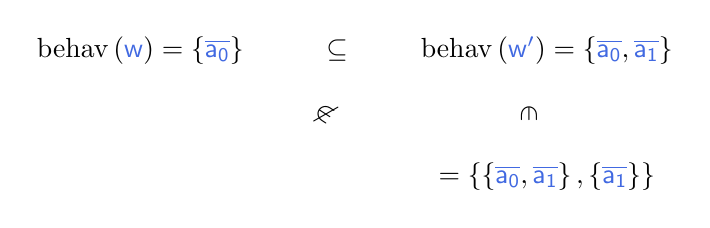
\begin{tikzpicture}
  \node (a) {$\behav{\src{\wholeprogvar}}=\left\{\src{\trace[_0]}\right\}$};
  \node[right=2cm of a] (b) {$\behav{\src{\wholeprogvar[']}}=\left\{\src{\trace[_0]},\src{\trace[_1]}\right\}$};
  \node[below=1cm of b] (d) {$\varHProp=\left\{\left\{\src{\trace[_0]},\src{\trace[_1]}\right\},\left\{\src{\trace[_1]}\right\}\right\}$};

  \node[right=.8cm of a] (ab) {$\subseteq$};
  \node[below=.5cm of b,rotate=270] (bd) {$\in$};
  \node[below=.3cm of ab,rotate=-33] (ad) {$\not\in$};
\end{tikzpicture}
\end{center}

Clearly, $\operatorname{behav}(\src{\wholeprogvar})\subseteq\operatorname{behav}(\src{\wholeprogvar'})$, so $\src{\wholeprogvar}$ {\em refines} $\src{\wholeprogvar'}$.
However, while $\src{\wholeprogvar[']}$ satisfies $\varHProp$ ($\sat{\src{\wholeprogvar[']}}{\varHProp}$), we have that $\not\sat{\src{\wholeprogvar}}{\varHProp}$.
This does not break for ordinary trace-based properties, since refinement coincides with satisfaction, i.e., taking subsets is a transitive operation.






\section{Secure Composition}\label{sec:sequential}

Notably, real-world compilation chains also perform a series of (sequential) passes whose main purpose is not necessarily to translate from one language to another, but to, e.g., optimise the code or enforce a certain property.
Both examples can be seen in practice, e.g.,~\cite{nagarakatte2009soft,nagarakatte2010cets,akritidis2009baggy,wegman1991ccp,manjikian1997fusion} and many more.
% \MPin{survey to cite? this is a bit informal MK: hard to find a survey on different compiler passes... I can't even find one just for compiler enforced memsafety (that looks good) or for compiler translations in general}.
% 
% Consider the compilation passes of LLVM~\cite{lattner2004llvm}, which are handled in the \texttt{PassManager} class.
% By manipulating the internal state of a \texttt{PassManager} object, the schedule of compiler optimisation passes can be hardcoded.
% That way, an order of optimisations can be found by hand that yields the best results.
% \MP{what's the point of the previous 3 sentences?(commented)}
Consider the following two LLVM optimisation passes: \gls*{cf}, which rewrites constant expressions to the constant they evaluate to, and \gls*{dce}, which removes dead code by rewriting conditional branches.
The order in which \gls*{cf} and \gls*{dce} are performed influences the final result of the compilation (see \Cref{fig:cfdceex}).
\begin{figure}[!ht]
  \begin{center}
    \begin{tikzpicture}[scale=0.62, every node/.style={transform shape}]
      \node[minimum width=3cm,minimum height=2.5cm,draw=black,very thick,align=left] (progunopt) {\begin{lstlisting}[language=ml,basicstyle=\small\ttfamily]
let a = true in
if a then
  print "a"
else
  print "b"
\end{lstlisting}};
      \node[minimum width=3cm,minimum height=2.5cm,draw=black,very thick,align=left,right=1.0 of progunopt] (progoptcf) {\begin{lstlisting}[language=ml,basicstyle=\large\ttfamily]
if true then
  print "a"
else
  print "b"
\end{lstlisting}};
      \node[minimum width=3cm,minimum height=2.5cm,draw=black,very thick,align=left,right=1.0 of progoptcf] (progoptcfdce) {\begin{lstlisting}[language=ml,basicstyle=\Large\ttfamily]
print "a"
\end{lstlisting}};% the following is a hack to get my syntax highlighting to work again \end{lstlisting}
      % edges
      \draw[->,very thick] (progunopt) edge[loop left,left] node {\gls*{dce}} (progunopt);
      \draw[->,very thick] (progunopt) edge[sloped,above] node {\gls*{cf}} (progoptcf);
      \draw[->,very thick] (progoptcf) edge[sloped,above] node {\gls*{dce}} (progoptcfdce);
    \end{tikzpicture}
  \end{center}
  \caption{Example program where the level of optimisations differ for one pass of applying \gls*{cf} and \gls*{dce} in any order. %
  Every edge is a compilation pass and the label on the edge states what the pass does, i.e., \gls*{cf} or \gls*{dce}. %
  The source code in the nodes is a glorified compiler intermediate representation and the code gets more optimised towards the right hand side of the figure.}\label{fig:cfdceex}
\end{figure}
This {\em phase ordering problem} is well--known in literature and a practical solution is to simply perform a fixpoint iteration of the optimisation pipeline~\cite{click1995combining}.

\smallskip

To analyse the security of compilation passes and their interaction within a compilation pipeline, we rely on a few key notions: the definition of a trace relation, and the definition of when is a trace relation well-formed with respect to a class.
%
Consider traces $\src{\trace}$ and $\trg{\trace}$ as well as two trace relations $\sim_1$ and $\sim_2$. 
% 
The traces are related $\src{\trace}\sim_1\bullet\sim_2\trg{\trace}$ if there is another trace $\irl{\trace}$ such that $\src{\trace}\sim_1\irl{\trace}$ and $\irl{\trace}\sim_2\trg{\trace}$.
% 
\bul{A relation $\sim$ is well-formed w.r.t. a class of target-level properties $\trg{\class}$} iff \rul{the universal image preserves set membership}.
\begin{definition}[Well-formedness of $\sim$ for a Class $\trg{\class}$]\label{def:wfc:sig:tracerel}
  % $$

  \begin{nscenter}
  \noindent
  \text{\bul{$\wfcsig{\sim}{\trg{\class}}$}} \isdef \text{\rul{$\forall \trg{\pi}\in\trg{\class}, \sigma_\sim(\trg{\pi})\in\sigma_\sim(\trg{\class})$}}
  \end{nscenter}
  % $$
\end{definition}

We can now state our main result: secure compilers in the robust compilation framework~\cite{abate2021extacc} compose {\em sequentially}. 
% 




Let \bul{$\cc{\src{L}}{\trg{L}}$ robustly preserve the class $\sigma_{\sim_2}\left(\obj{\class[_1]}\right)$ under $\sim_1$} and let \rul{$\cc{\trg{L}}{\obj{L}}$ robustly preserve the class $\obj{\class[_2]}$ under $\sim_2$}.
Then, \iul{when the cross-language relation $\sim_2$ is well-formed w.r.t. class $\obj{\class[_1]}$}, it follows that \oul{the composed compiler\footnote{Here, $\cc{\src{L}}{\trg{L}}\circ\cc{\trg{L}}{\obj{L}}$ means first running $\cc{\src{L}}{\trg{L}}$ and then $\cc{\trg{L}}{\obj{L}}$.} $\cc{\src{L}}{\trg{L}}\circ\cc{\trg{L}}{\obj{L}}$ robustly preserves the intersection of classes $\obj{\class[_1]}\cap\obj{\class[_2]}$ under $\sim_1\bullet\sim_2$}.
% 
%For space reasons, \Thmref{thm:urtp} and \Thmref{thm:lrtp} are not presented here, but can be found in the technical appendix ($\CoqSymbol$).
% Note that it is not necessary to require $\sim_2$ to be well-formed w.r.t. $\src{\class[_1]}$, since the 
% \MPin{why}
\begin{theorem}[Composition of Secure Compilers w.r.t. $\sigma$]\label{thm:rtpsim:sig}
  $\;$ 

  If \bul{$\rtpsig{\cc{\src{L}}{\trg{L}}}{\tilde{\sigma}_{\sim_2}\left(\obj{\class[_{1}]}\right)}{\sim_1}$}, \rul{$\rtpsig{\cc{\trg{L}}{\obj{L}}}{\obj{\class[_2]}}{\sim_2}$}, and \iul{$\wfcsig{\sim_2}{\obj{\class[_1]}}$}, \\ then \oul{$\rtpsig{\cc{\src{L}}{\trg{L}}\circ\cc{\trg{L}}{\obj{L}}}{\obj{\class[_{1}]}\cap\obj{\class[_{2}]}}{\sim_1\bullet\sim_2}$}. \Coqed
\end{theorem}

Since the composition of secure compilers is again a secure compiler, the theorems generalise to a whole chain of $n$ secure compilers. 
% 
\Cref{thm:rtpsim:sig} can also be stated for the existential image $\tau_\sim\left(\src{\pi}\right)$, but in the interest of space that result has been moved to the appendix.
 % (\Cref{subsec:extimg}).
% 
Crucially, \Cref{thm:rtpsim:sig} also holds for \emph{classes of hyperproperties}, and thus, compilers that robustly preserve hyperproperties can be composed with each other as well as with compilers that robustly preserve properties.
% 
%Unfortunately, proofs of compilers that robustly preserve hyperproperties (including hypersafety) are scarce in the literature due to their complexity.
%\MP{ so what ? }
%  we don't discuss this further?
% 

% It is furthermore possible to conflate the notion of classes and hyperproperties by intersecting all elements of a class of hyperproperties, to obtain one combined hyperproperty.
% This idea has been discussed in other work~\cite{clarkson2008hyper}.
%  MP: i think i stated the point of these 2 lines above

If we take SecurePtrs and FaCT from \Cref{subsec:bg:rtp} and compose them according to \Cref{thm:rtpsim:sig}, we obtain a compiler that robustly preserves the intersection of safety properties and the \gls*{cct} hyperproperty. 
That is, for a source component that robustly satisfies any set of safety properties {\em and} \gls*{cct}, the compiled target component also robustly satisfies the same set of safety properties and \gls*{cct}.
% The intersection simply uses the lifted version of the respective safety properties.
%\MP{meaning?}

Compiler engineers typically try to find an order of optimisations that yields well-optimised programs for either code size~\cite{cooper1999geneticphases} or performance~\cite{kulkarni2006exhaustivephase}.
\Cref{corr:swappable} justifies that any such order of compilation passes is valid w.r.t. security, as long as the trace-relations have no effect on the respective classes.

So, given two compilation passes \bul{$\cc[_{1}]{\trg{L}}{\trg{L}}$, $\cc[_{2}]{\trg{L}}{\trg{L}}$, both robustly preserving class $\trg{\class[_{1}]}$ or $\trg{\class[_{2}]}$, respectively}, \rul{their corresponding well-formed trace-relations}, \iul{and indifference of the classes with respect to these trace relations}, \oul{for any order of their composition, the composed compiler robustly preserves the intersection of $\trg{\class[_{1}]}$ and $\trg{\class[_{2}]}$}.
% 
% \MPin{
% 	later on, say that optimisation passes remove elements from traces, so they should be fine w.r.t. the result with $\tau$.
% 	also, yes, if $\tau$ adds we have a problem, if it removes we don't
% \MKin{ Optimisations that remove elements from traces are not necessarily sound,
%  e.g., remove all deallocations to "optimise" memory management by offloading
%  the work to the OS.
% }
% }

\begin{corollary}[Swapping Secure Compiler Passes]\label{corr:swappable}
  $\;$ 

  If \bul{$\rtpsig{\cc[_{1}]{\trg{L}}{\trg{L}}}{\trg{\class[_{1}]}}{\sim_1}$ and $\rtpsig{\cc[_{2}]{\trg{L}}{\trg{L}}}{\trg{\class[_{2}]}}{\sim_2}$}, %
  \rul{$\wfcsig{\sim_1}{\trg{\class[_2]}}$ and $\wfcsig{\sim_2}{\trg{\class[_1]}}$}, %
  and \iul{$\tilde{\sigma}_{\sim_2}\left(\trg{\class[_1]}\right)=\trg{\class[_1]}$ as well as $\tilde{\sigma}_{\sim_1}\left(\trg{\class[_2]}\right)=\trg{\class[_2]}$},
  then \oul{$\rtpsig{\cc[_{1}]{\trg{L}}{\trg{L}}\circ\cc[_{2}]{\trg{L}}{\trg{L}}}{\trg{\class[_{1}]}\cap\trg{\class[_{2}]}}{\sim_1\circ\sim_2}$ and $\rtpsig{\cc[_{2}]{\trg{L}}{\trg{L}}\circ\cc[_{1}]{\trg{L}}{\trg{L}}}{\trg{\class[_{2}]}\cap\trg{\class[_{1}]}}{\sim_2\circ\sim_1}$}. \Coqed
\end{corollary}

Coming back to the example composing SecurePtrs with FaCT, it is likely the case that \Cref{corr:swappable} is not applicable.
While first running SecurePtrs and then FaCT should be fine, the other direction has potential security hazards, since the SecurePtrs compiler does not account for cryptographic-constant time primitives, such as \texttt{ctselect}.

\subsection{Secure Compiler Composition with Same Trace Models}
When the cross-language trace relation is an equality, \Cref{thm:rtpsim:sig} collapses:
Given \bul{$\cc{\src{L}}{\trg{L}}$ robustly preserves $\class[_{1}]$} and \rul{$\cc{\trg{L}}{\obj{L}}$ robustly preserves $\class[_{2}]$}, it follows that \oul{their sequential composition $\cc{\src{L}}{\trg{L}}\circ\cc{\trg{L}}{\obj{L}}$ robustly preserves the intersection of classes $\class[_{1}]$ and $\class[_{2}]$}.

\begin{corollary}[Composition of Secure Compilers]\label{corr:rtp}
  $\;$ 

  If \bul{$\rtp{\cc{\src{L}}{\trg{L}}}{\class[_{1}]}$} and \rul{$\rtp{\cc{\trg{L}}{\obj{L}}}{\class[_{2}]}$}, then \oul{$\rtp{\cc{\src{L}}{\trg{L}}\circ\cc{\trg{L}}{\obj{L}}}{\class[_{1}]\cap\class[_{2}]}$}. \Coqed
\end{corollary}

\Cref{corr:rtp} provides an easy way to compose secure compilers without well-formedness of trace relations. 
% 
However, while \Cref{thm:rtpsim:sig} explicitly requires that $\sim_1$ is well-formed w.r.t. $\trg{\class[_2]}$, if $\sim_2$ is not well-formed w.r.t. $\trg{\class[_1]}$, care must be taken. 
%Worst-case is that the resulting class $\sigma_{\sim_1\bullet\sim_2}\left(\trg{\class[_1]}\cap\trg{\class[_2]}\right)$ becomes empty, even though $\trg{\class[_1]}\cap\trg{\class[_2]}$ is not necessarily empty.
This is further discussed in \Cref{subsec:compatsecpasses}.

%If possible, optimisations are merged to enhance the analysis' result, since even when iterating to a fixpoint the final program may not be as optimised as it could be~\cite{click1995combining}.
We can also obtain a specialised version of \Cref{corr:swappable}:
%So, given two compilation passes \bul{$\cc[_{1}]{\trg{L}}{\trg{L}}$, $\cc[_{2}]{\trg{L}}{\trg{L}}$, both robustly preserving class $\class[_{1}]$ or $\class[_{2}]$, respectively}, \oul{for any order of their composition, the composed compiler robustly preserves the intersection of $\class[_{1}]$ and $\class[_{2}]$}.
% 
% \MPin{
% 	later on, say that optimisation passes remove elements from traces, so they should be fine w.r.t. the result with $\tau$.
% 	also, yes, if $\tau$ adds we have a problem, if it removes we don't
% \MKin{ Optimisations that remove elements from traces are not necessarily sound,
%  e.g., remove all deallocations to "optimise" memory management by offloading
%  the work to the OS.
% }
% }

\begin{corollary}[Swapping Secure Compiler Passes]\label{corr:swappable:one}
  $\;$ 

  If {$\rtp{\cc[_{1}]{\trg{L}}{\trg{L}}}{\class[_{1}]}$ and $\rtp{\cc[_{2}]{\trg{L}}{\trg{L}}}{\class[_{2}]}$}, then {$\rtp{\cc[_{1}]{\trg{L}}{\trg{L}}\circ\cc[_{2}]{\trg{L}}{\trg{L}}}{\class[_{1}]\cap\class[_{2}]}$ and $\rtp{\cc[_{2}]{\trg{L}}{\trg{L}}\circ\cc[_{1}]{\trg{L}}{\trg{L}}}{\class[_{2}]\cap\class[_{1}]}$}. \Coqed
\end{corollary}

\section{Security Properties Formalisation \& Composition\pages{1.5}}\label{sec:compprop}

This section introduces trace properties of interest for this paper: \gls*{tms}, \gls*{sms}, \gls*{ms}, \gls*{scct}, and \gls*{ss}.
These properties are of practical importance (as mentioned in \Cref{sec:introduction}) and also of interest in the case study presented later (\Cref{sec:casestud:defs,sec:casestud:rtp}). 
This section presents all of them, despite the fact that they are inspired by existing work, in order to showcase all that is required for a formal proof of security for a realistic compilation toolchain.
%\MP{ say something about this in the rebuttal: only the defs are borrowed, the universal images and all that work is new}
%\MK{ universal images are not new. }
% , none of the properties is novel, for self-containment of the paper, their definition is necessary for the case study.
% For each of the presented properties, the technical report defines corresponding monitors, which refine a given property and have a key role in the proofs of this paper. 
The technical report defines monitors for each of the presented properties.
% 
Monitors refine each property and have a key role in the proofs of this paper.
% managed to prove 
%  if tms-monitor --[trace]-->* ∅  
%  then trace ∈ tms
% but not
%  if trace ∈ tms
%  then tms-monitor --[trace]-->* ∅

\subsection{A Trace Model for Memory Safety}\label{subsec:basic:memsafety:tracemodel}

For simple memory safety composed of temporal and spatial memory safety, the trace model defines events ($\event[_{\mssafe}]$) as either the empty event ($\emptyevent$), a crash ($\lightning$), or a base-event ($\preevent[_{\mssafe}]$).

\vspace{-1.0em}
\[
  \begin{array}{rcll}
    \text{(Base-Events)}&\preevent[_{\mssafe}] &:=& \ev{Alloc \loc\ n} \mid \ev{Dealloc \loc} \mid \ev{Use \loc\ n} \\
    \text{(Events)}&\event[_{\mssafe}] &:=& \preevent[_{\mssafe}] \mid \emptyevent \mid \lightning \\ 
  \end{array}
\]

Base-events describe the actual kind of event that happened.
For the basic memory-safety properties, these are three variants:
First, the allocation event ($\ev{Alloc\ \loc\ n}$) that fires whenever a program claims $n$ cells of memory and stores them at address $\loc$, where addresses are assumed to be unique.
Second, deallocation ($\ev{Dealloc\ \loc}$) announces that the object at location $\loc$ is freed.
Third, an event to describe reads from and writes to the $n$-th memory cell from address $\loc$ ($\ev{Use\ \loc\ n}$).

\subsubsection{Temporal Memory Safety}

\gls*{tms}~\cite{nagarakatte2010cets} is a safety property that describes that an unallocated object must not be (re-)used.

\begin{definition}[\glsfirst*{tms}]\label{def:trace:tmsdef}
  % \footnotesize
  $$
  \tmssafe:=\left\{\trace[_{\mssafe}] \left| \begin{array}{rcl}
    \ev{Alloc\ \loc\ n}&\le_{\trace[_{\mssafe}]}&\ev{Dealloc\ \loc} \\
    \ev{Use\ \loc\ n}&\le_{\trace[_{\mssafe}]}&\ev{Dealloc\ \loc} \\
    \text{at most one }\ev{Dealloc\ \loc}&\text{in}&\trace[_{\mssafe}] \\
    \text{at most one }\ev{Alloc\ \loc\ n}&\text{in}&\trace[_{\mssafe}] \\
  \end{array}\right.\right\}
  $$
\end{definition}
Hereby, the notation $\event[_{1}]\le_{\trace}\event[_{2}]$ means that if $\event[_{1}]$ is in $\trace$ and if $\event[_{2}]$ is in $\trace$, then $\event[_{1}]$ appears before $\event[_{2}]$.

\subsubsection{Spatial Memory Safety}

\gls*{sms}~\cite{nagarakatte2009soft} is a safety property that prohibits out-of-bounds accesses.

\begin{definition}[\glsfirst*{sms}]\label{def:trace:smsdef}
% \small
  % \begin{nscenter}

  \noindent
  \[
  \smssafe:=\left\{\trace[_{\mssafe}] \left|\begin{array}{rcl}
      \text{If }\ev{Alloc\ \loc\ n}\le_{\trace_{\mssafe}}\ev{Use\ \loc\ m}, \text{ then }m<n
  \end{array}\right.\right\}
  \]
  % \end{nscenter}
\end{definition}

\subsubsection{Memory Safety}

In spirit of earlier work~\cite{nagarakatte2009soft,nagarakatte2010cets,jim2002cyclone,necula2005ccured,michael2023mswasm}, full \gls*{ms} is the intersection of \Cref{def:trace:tmsdef,def:trace:smsdef}.

\begin{definition}[\glsfirst*{ms}]\label{def:trace:msdef}
  $
  \mssafe:=\tmssafe \cap \smssafe
  $
\end{definition}

Note that \Cref{def:trace:msdef} ignores data isolation, so there may still be memory-safety issues introduced by side-channels.

\subsection{A Trace Model for Memory Safety with Constant Time}\label{subsec:scct:tracemodel}

To express Constant Time, we extend the memory safety trace model with a {\em security tag} ($\securitytag{}$) that indicates whether events contain sensitive information ($\lock$) or not ($\unlock$).

\vspace{-.5em}
\[
  \begin{array}{rrcl}
    (\text{Base-Events}) & \preevent[_{\ctsafe}] &:=& \preevent[_{\mssafe}] \mid \ev{Branch\ }n \mid \ev{Binop\ }n\\
    (\text{Security Tags}) & \securitytag{} &:=& \lock \mid \unlock\\ 
    (\text{Events}) & \event[_{\ctsafe}] &:=& \preevent[_{\ctsafe}];\securitytag{} \mid \emptyevent \mid \lightning \\ 
  \end{array}
\]

For cryptographic code, there is a general guideline that secrets must not be visible on a trace~\cite{ctguidelines}, i.e., secrets should not be marked as $\unlock$.
In turn, an instruction whose timing is data-dependent must not have a secret as an operand.
Typical operations with data-dependent timing are branches and certain binary operations, such as division.%
\footnote{
	This is architecture-dependent, but division is an operation that serves as a classic example for a data-dependent timing instruction~\cite[p.~755]{arm-refman}.
}
Both operations are represented in the trace model by extending the set of base-events with branches ($\ev{Branch\ n}$) and binary operations ($\ev{Binop\ n}$).

\subsubsection{Strict Cryptographic Constant Time}

\gls*{cct} is a hypersafety property~\cite{barthe2018sec} and, thus, difficult to check with monitors.
This is because, intuitively, hypersafety properties can relate multiple execution traces with each other, but monitors work on a single execution.
It is a common trick to sidestep this issue by means of overapproximation: this section defines the property \gls*{scct}, a stricter variant of \gls*{cct} (inspired by earlier work~\cite{almeida2017jasmin}) that enforces the policy that no secret appears on a trace.
Programs that satisfy \gls*{scct} also satisfy \gls*{cct}, but programs that satisfy \gls*{cct} may not satisfy \gls*{scct}.

\begin{definition}[\glsfirst*{scct}]\label{def:trace:scctdef}
% \begin{nscenter}
  
  \noindent\[
  \scctsafe:=\left\{\trace[_{\ctsafe}] \left|\begin{array}{l}
      \trace[_{\ctsafe}]=\hole{\cdot} \text{ or } \\\exists\trace[_{\ctsafe}'],\trace[_{\ctsafe}]=\preevent[_{\ctsafe}];\unlock\cdot\trace[_{\ctsafe}'] \wedge \trace[_{\ctsafe}']\in\scctsafe
    \end{array}\right.\right\}
  \]
% \end{nscenter}
\end{definition}

\gls*{scct} may appear overly strict, since it seems that secrets must not occur on a trace (since $\securitytag{}$ is forced to be $\unlock$). 
However, this is considered standard practice in terms of coding guidelines~\cite{ctguidelines}.
Moreover, programs that have been compiled with FaCT~\cite{cauligi2019fact} and run with a ``data independent timing mode''~\cite{arm-refman,intel-refman} enabled do not leak secrets (see \Cref{ex:lscct}). 

\subsubsection{\gls*{ms}, Strict Cryptographic Constant Time}\label{sec:msscct-rel}

The combination of \gls*{ms} and \gls*{scct} is the intersection of these properties, \gls*{msscct}.
However, \gls*{ms} uses a different trace model than \gls*{scct}, so intersecting them would trivially yield the empty set. 
To remedy this issue, we introduce $\sim_{\ctsafe}: \preevent[_{\ctsafe}] \times \preevent[_{\mssafe}] $, a cross-language trace relation (whose key cases are presented below), that we use to intuitively unify the trace model in which the two properties are expressed:
\[
  \typerulenolabel{mscctrel:drop:tag}{}{\preevent[_{\mssafe}]\sim_{\ctsafe}\preevent[_{\mssafe}];\unlock{}}
  \typerulenolabel{mscctrel:drop:crash}{}{\lightning\sim_{\ctsafe}\lightning}
\]
\[
  \typerulenolabel{mscctrel:drop:branch}{}{\emptyevent\sim_{\ctsafe}\ev{Branch n};\securitytag{}}
  \typerulenolabel{mscctrel:drop:binop}{}{\emptyevent\sim_{\ctsafe}\ev{Binop n};\securitytag{}}
\]

Essentially, $\sim_{\ctsafe}$ ignores both the new $\ev{Branch\ n}$ and $\ev{Binop\ n}$ base-events as it relates security-insensitive actions ($\unlock$) to their equivalent counterparts.
Thus, \gls*{ms} traces trivially satisfy \gls*{scct}.
% 
The above relation is extended point-wise to traces, skipping the empty event $\emptyevent$ on either side, and it is now possible to define \gls*{msscct} using the universal image:

\begin{definition}[\gls*{ms} and \gls*{scct}]\label{def:trace:msscctdef}
  $
  \msscctsafe:=\mssafe\cap\sigma_{\sim_{\ctsafe}}\left(\scctsafe\right)
  $
\end{definition}

\subsection{Extending the Trace Model with Speculation}\label{subsec:msctss:tracemodel}

So far, the considered trace models do not let us express speculative execution attacks such as Spectre~\cite{kocher2019spectre}. 
For this, we extend the earlier trace model (see \Cref{subsec:scct:tracemodel}) so that the security tags ($\securitytag{}$) carry additional information about the kind of private data leakage, i.e., the type of speculative leak.
Moreover, we add base-events signalling the beginning of a speculative execution ($\ev{Spec}$), a barrier ($\ev{Barrier}$) that signals that any speculative execution may not go past it, as well as a rollback event ($\ev{Rlb}$), which signals that execution resumes to where speculation started.

\vspace{-1em}
{
\[
  \begin{array}{rrcl}
    (\text{Base-Events}) & \preevent[_{\mathghost}] &:=& \preevent[_{\ctsafe}] \\
    (\text{Spectre Variants}) & vX &:=& \operatorname{NONE} \mid \operatorname{PHT} \\
    (\text{Security Tags}) & \securitytag{} &:=& \lock_{vX} \mid \unlock\\ 
    (\text{Events}) & \event[_{\mathghost}] &:=& \preevent[_{\mathghost}];\securitytag{} \mid \emptyevent \mid \lightning \mid \ev{Spec} \mid \ev{Rlb} \mid \ev{Barrier}\\ 
  \end{array}
\]
}

Even though the considered Spectre variants are just SPECTRE-PHT~\cite{kocher2019spectre}, NONE just describes secret data as in \gls*{scct} (see \Cref{subsec:scct:tracemodel}), the trace model is general enough to allow for potential future extension with different variants~\cite{kocher2019spectre,maisuradze2018ret2spec,horn2019zero}.
%For sake of readability, this paper just uses the notation $\lock$ in place of $\lock_{\text{PHT}}$.

\subsubsection{Speculative Safety}

\gls*{ss}~\cite{patrignani2021exorcising}, similar to \gls*{scct}, is a sound overapproximation of a variant of noninterference.

\begin{definition}[\glsfirst*{ss}]\label{def:trace:ss}
  \noindent

  \begin{nscenter}
  $
    \sssafe:=\left\{\trace[_{\mathghost}] \left|\begin{array}{l}
      \trace[_{\mathghost}]=\hole{\cdot} \text{ or } \exists\trace[_{\mathghost}'].\\
      \left(\trace[_{\mathghost}]=\preevent[_{\mathghost}];\unlock\cdot\trace[_{\mathghost}'] \text{or }\trace[_{\mathghost}]=\preevent[_{\mathghost}];\lock_{\text{NONE}}\cdot\trace[_{\mathghost}']\right)\\
      \text{and }\ \trace[_{\mathghost}']\in\sssafe
                                 \end{array}\right.\right\}
  $ 
  \end{nscenter}
\end{definition}
The technical setup so far leads to the above definition, where only locks annotated with $\text{SPECTRE-PHT}$ are disallowed to occur on the trace.
That way, programs attaining \gls*{ss} do not necessarily attain \gls*{scct}.

\subsubsection{Speculation Memory Safety}\label{sec:spec-ms-rel}

As before, we need to relate the different trace models with each other, so that the memory safety property without speculation can be lifted to speculation. 
To this end, let $\sim_{\mathghost}: \preevent[_{\mathghost}] \times \preevent[_{\ctsafe}]$ be a cross-language trace relation whose key cases are below.
The intuition is that \gls*{ss} is trivially satisfied in \gls*{scct}, since speculation is inexpressible there, which amounts to dropping events $\ev{Spec}$, $\ev{Rlb}$, or $\ev{Barrier}$, as well as all base events tagged with $\lock_{\text{PHT}}$. 

\[
  \typerulenolabel{specrel:drop:tag}{}{\preevent[_{\ctsafe}];\lock\sim_{\mathghost}\preevent[_{\mathghost}];\lock_{\text{NONE}}}
  \typerulenolabel{specrel:drop:spectag}{}{\emptyevent\sim_{\mathghost}\preevent[_{\mathghost}];\lock_{\text{PHT}}}
\]
\[
  \typerulenolabel{specrel:drop:pub}{}{\preevent[_{\ctsafe}];\unlock\sim_{\mathghost}\preevent[_{\mathghost}];\unlock}
  \typerulenolabel{specrel:drop:crash}{}{\lightning\sim_{\mathghost}\lightning}
\]
\[
  \typerulenolabel{specrel:drop:spec}{}{\emptyevent\sim_{\mathghost}\ev{Spec}}
  \typerulenolabel{specrel:drop:rlb}{}{\emptyevent\sim_{\mathghost}\ev{Rlb}}
  \typerulenolabel{specrel:drop:barrier}{}{\emptyevent\sim_{\mathghost}\ev{Barrier}}
\]

We conclude by defining the ultimate property of interest for secure compilers: \gls*{specms}.
\begin{definition}[\gls*{specms}]\label{def:trace:specmsdef}
  $
  \specmssafe := \msscctsafe\cap\sigma_{\sim_{\mathghost}}\left(\sssafe\right)
  $
\end{definition}






\section{Case Study: Language Formalisations\pages{2}}\label{sec:casestud:defs}

This section defines programming languages $\Ltms$, $\Ltrg$, $\Lms$, $\Lscct$, and $\Lspec$, all of which share common elements (presented in \Cref{subsec:cs:defs}).
$\Ltms$ is the only statically-typed language, and it exhibits the property that all well-typed programs are \gls*{tms} (\Cref{subsec:ltms}).
However, not all $\Ltms$ programs are \gls*{sms}.
That is, there are well-typed $\Ltms$ programs that perform an out-of-bounds access.
Language $\Ltrg$ is untyped and does not provide any guarantees with regards to \gls*{ms} (\Cref{subsec:lsms}).
$\Lms$ is exactly the same language as $\Ltrg$, but this paper still distinguishes the two for sake of readability (\Cref{subsec:lms}).
All three languages --- so $\Ltms$, $\Ltrg$, and $\Lms$ --- assume \gls*{scct} to hold, since this is -- in an ideal world -- what the programmer would expect, too: it is the job of the compiler to preserve and (potentially) enforce \gls*{scct} security~\cite{cauligi2019fact,nagarakatte2010cets,nagarakatte2009soft,akritidis2009baggy}.
% This paper considers \gls*{cct} as an architecture-dependent property\MPin{can we justify this}, so

Such consideration is also backed up by architecture providing a data (operand) independent timing mode, such as processors by Arm~\cite[p.~543]{arm-refman} and Intel~\cite[p.~80]{intel-refman}.
%In spirit of this, all languages besides $\Lscct$ are trivially \gls*{scct}. 
This kind of processor feature is modelled in language $\Lscct$ (\Cref{subsec:lscct}), where programs have access to a ``\gls*{cct}-mode'' and can change the leakage of emitted events according to the value of this mode (either $\obj{ON}$ or $\obj{OFF}$). 

Finally, modern processors also employ speculative execution to achieve speedups---and unfortunately generate Spectre attacks~\cite{kocher2019spectre}---and this is the extension of $\Lspec$ (\Cref{subsec:lspec}).
 % extends $\Lscct$ to model speculative execution.
%
Thus, all previous languages trivially satisfy \gls*{ss}, since they do not support speculative execution at all.
% All languages share large parts of syntactic elements, which are presented in the next subsection (\Cref{subsec:cs:defs}).
% Subsequent subsections extend on this accordingly.

\subsection{Shared Language Definitions}\label{subsec:cs:defs}

All presented programming languages share a common fragment which is partially presented here and in full detail in the technical report. 
%\MP{put omitted stuff in appendix + ref there (and add textual explanation)}

% \vspace{-.5em}
{
  \renewcommand{\src}[1]{\mathsf{#1}}
 \small
\[
  \begin{array}{rrcl}
    \text{(Base-Events)} & \src{\preevent} &:=& \src{\ev{Alloc \loc\ n}} \mid \src{\ev{Dealloc \loc}} \mid \src{\ev{Get \loc\ n}} \mid \src{\ev{Set \loc\ n}} \\
    \text{(Control Tags)} & \src{\sandboxtag{}} &:=& \src{\ctx} \mid \src{\comp} \\
    \text{(Events)} & \src{\event} &:=& \src{\preevent;\sandboxtag{}} \mid \src{\emptyevent} \mid \src{\lightning} \\ 
    \text{(Values)} & \src{v} &:=& \src{n} \\
    \text{(Expressions)} & \src{\expr} &:=& \src{x} \mid \src{n} \mid \src{\lbinop{\expr[_1]}{\expr[_2]}} \mid \src{\lifz{\expr[_1]}{\expr[_2]}{\expr[_3]}} \\ 
                         &&&\mid \src{\llet{x}{\expr[_1]}{\expr[_2]}} \mid \src{\llet{x}{new\ \expr[_1]}{\expr[_2]}} \\
                         &&&\mid \src{\ldelete{x}} \mid \src{\lget{x}{\expr}} \mid \src{\lset{x}{\expr[_1]}{\expr[]}} \mid \src{stuck}\\
                         &&&\mid \src{\lcall{f}{\expr}} \mid \src{\lreturn{\expr}} \\
    \text{(Functions)} & \src{F} &:=& (\src{x};\src{\expr}) \\
    \text{(Libraries)} &&&\hspace{-3.8em} \src{\library_{\ctx}},\src{\library_{\comp}} : \src{Vars} \to \src{F} 
    % \hspace{2em}
    %  : \src{Vars} \to \src{F} 
     \\
    \text{(Heaps)} & \src{H} &:=& \src{\hole{\cdot}} \mid \src{n},\src{H}
    % \hspace{0.5cm}    
    \\
    \text{(Pointer Maps)} & \src{\Delta} && \text{ omitted for simplicity}
    \\
    \text{(Memory States)} & \src{\memstate} &:=& \left(\src{H^{\ctx}};\src{H^{\comp}};\src{\Delta}\right)\\
    \text{(Control States)} & \src{\cfstate} & & \text{ omitted for simplicity} 
    \\
    \text{(States)} &\src{\Omega} &:=& \left(\src{\cfstate};\src{\sandboxtag{}};\src{\memstate}\right)\\
  \end{array}
\]
}
{
  \renewcommand{\src}[1]{\mathsf{#1}}
The trace models of all languages are similar to those presented earlier (\Cref{sec:compprop}).
One technical detail is the addition of a control tag, indicating who is to blame for an emitted action: context ($\ctx$) or component ($\comp$).
This is a standard technique in secure compilation in order to rule out irrelevant context-level events. 
For example, a context immediately deallocating an allocated memory region twice trivially violates memory safety, but the main interest in secure compilation is to preserve component-level security, and thus component events.
Even though this tagging could be used for blame preservation~\cite{patrignani2023blame}, this is beyond the focus of this paper.
Another key difference is that memory accesses are now explicitly modelled as reads ($\src{\ev{Read\ \loc\ n}}$) and writes ($\src{\ev{Write\ \loc\ n}}$) instead of just uses.

All languages have at least numbers as values ($\src{v}$) and second class functions ($\src{F}$).
Functions are modelled as pairs containing the name of one argument and the body of the function.
Bodies are just ordinary expressions, which can be simple binary operations ($\src{\lbinop{\expr[_1]}{\expr[_2]}}$), conditionals ($\src{\lifz{\expr[_1]}{\expr[_2]}{\expr[_3]}}$), function calls ($\src{\lcall{f}{e}}$) and returns ($\src{\lreturn{\expr}}$), as well as C-like memory operations. 
Programs have sets of pre-determined functions called libraries and they are marked as being part of some component ($\src{\library_{\comp}}$) or context ($\src{\library_{\ctx}}$).

For the operational semantics, the runtime state ($\src{\Omega}$) is a triple consisting of a control-flow state ($\src{\cfstate}$), a control tag ($\src{\sandboxtag{}}$), and a memory state ($\src{\memstate}$). 
The latter carries information about pointers that are kept ``alive'' in pointer maps ($\src{\Delta}$), so that the semantics does not get stuck when encountering, e.g., a double-free.
The memory state also carries two heaps to model sandboxing between a context ($\src{H^{\ctx}}$) and a component ($\src{H^{\comp}}$).

}

\subsection{$\src{L_{\tmssafe}}$: A Temporal but Not Spatial Memory Safe Language}\label{subsec:ltms}

$\src{L_{\tmssafe}}$ is the only statically-typed language in this case study and restricts functions ($\src{F}$) to the typing signature $\src{\natt\to\natt}$. 
The type system of $\src{L_{\tmssafe}}$ is inspired by $L^{3}$~\cite{morrisett2005L3,scherer2018fabulous} and enforces that every well-typed $\src{L_{\tmssafe}}$ program satisfies \gls*{tms}.
 % (\Cref{thm:wt:tms}).

\begin{theorem}[$\src{L_{\tmssafe}}$-programs are \gls*{tms}]\label{thm:wt:tms}
$\rsat{\src{\library_{\comp}}}{\tmssafe}$ \Coqed
  % $\;$ 
% 
  % \begin{nscenter}
  %   \hfill For any component $\src{\library_{\comp}}$, $\rsat{\src{\library_{\comp}}}{\tmssafe}$ \Coqed
  % \end{nscenter}
\end{theorem}

\subsection{$\Ltrg$: A Memory-Unsafe Language}\label{subsec:lsms}

$\Ltrg$ extends the syntax presented earlier (\Cref{subsec:cs:defs}) with dynamic typechecks ($\trg{\lhast{\expr}{\type}}$), evaluating to $\trg{0}$ if the type matches with the shape of $\trg{\expr}$ and $\trg{1}$ otherwise.
%The pointers carry poison tags, which signify a pointer being allocated ($\trg{\poisoned}$) or freed ($\trg{\poisonless}$). 
Furthermore, the syntax of $\Ltrg$ is extended with a way to inspect whether a pointer is freed ($\trg{\lispoisoned{x}}$), evaluating to $\trg{0}$ if it is freed and to $\trg{1}$ otherwise.
Functions may receive arguments that are not $\trg{\natt}$, values are extended with tuples, and expressions are also extended with pair projections.

% \vspace{-1em}
\[
  \begin{array}{rrcl}
    \text{(Values)} & \trg{v} &:=& \dots \mid \trg{\lpair{v_1}{v_2}} \\
    \text{(Expressions)} & \trg{\expr} &:=& \dots \mid \trg{\lhast{\expr}{\tau}} \mid \trg{\lispoisoned{x}} \mid \trg{e.1} \mid \trg{e.2}
  \end{array}
\]

No changes are done to the trace model, but $\Ltrg$ has no static typing, making double-free code patterns possible.

\subsection{$\Lms$: Another Memory-Unsafe Language}\label{subsec:lms}
$\Lms$ is exactly equal to $\Ltrg$ (\Cref{subsec:lsms}), but used to emphasize that this is code after applying $\cc{\Ltrg}{\Lms}$ (\Cref{subsec:cs:ms}).

\subsection{$\Lscct$: A Memory-Unsafe Language with a Constant Time Mode}\label{subsec:lscct}

$\Lscct$ extends $\Lms$ (\Cref{subsec:lms}) with a ,,constant-time mode''. 
The activation of the mode can be checked ($\obj{\lrddoit{x}{\expr}}$), changed ($\obj{\lwrdoit{D}}$), and is stored in program states ($\obj{\Omega}$).
At the beginning of program execution of $\Lscct$ programs, the mode is turned off ($\obj{OFF}$).
If the mode is enabled (i.e., set to $\obj{ON}$), the intuition is that no secrets are leaked. 
This models the real-world\footnote{As present in Intel~\cite[p.80]{intel-refman} and ARM~\cite[p.~543]{arm-refman} processors.} data-independent timing mode as well as the result of compiling a program with FaCT~\cite{cauligi2019fact}.
For example, FaCT rewrite code that branches to use a constant-time selection primitive.
To not obfuscate our formalisation unnecessarily by duplicating syntax, we simply added the ,,constant-time mode'' to $\Lscct$.

% $\Lscct$ extends $\Lms$ (\Cref{subsec:lms}) with a way to read from ($\obj{\lrddoit{x}{\expr}}$) and to write to ($\obj{\lwrdoit{D}}$) a model-specific register that controls a constant-time mode. 
% This language is a combination of the effect of the FaCT compiler~\cite{cauligi2019fact} as well as a data-independent timing mode, a feature that is present in both Arm~\cite[p.~543]{arm-refman} and Intel~\cite[p.~80]{intel-refman} processors.
% \MP{ can we be more specific about the fact pass? }
% To this end, states ($\obj{\Omega}$) are extended with the value of the register ($\obj{D}$), which is initially set to be not active ($\obj{OFF}$).
% If the register is marked active ($\obj{ON}$), the intuition is that no secrets can appear on specification traces.
% If the register is marked inactive, secrets may appear on traces.
% The state of the register can be read and written to, e.g., \Cref{tr:e-wrdoit-off}.
% For the other languages seen earlier, the mode is intuitively always-on, i.e., the mode of execution always uses constant-time mode.

% \vspace{-.5em}
\[
  \begin{array}{rrcl}
    \text{(Mode Values)} & \obj{D} &:=& \obj{ON} \mid \obj{OFF} \\
    \text{(Security Tags)} & \obj{\securitytag{}} &:=& \obj{\lock} \mid \obj{\unlock} \\
    \text{(Base-Events)} & \obj{\preevent} &:=& \dots \mid \obj{iGet\ \loc\ v} \mid \obj{iSet\ \loc\ v} \\
                       &&& \mid\ \obj{Binop\ n} \mid \obj{Branch\ n} \\
    \text{(Events)} & \obj{\event} &:=& \obj{\preevent;\sandboxtag{};\securitytag{}} \mid \obj{\emptyevent} \mid \obj{\lightning} \\
    \text{(Expressions)} & \obj{\expr} &:=& \dots \mid \obj{\lrddoit{x}{\expr}} \mid \obj{\lwrdoit{D}} \\
                         &&&\mid\ \obj{\llet{x^{\securitytag{}}}{\expr[_1]}{\expr[_2]}}\\
    \text{(States)} & \obj{\Omega} & := & \left(\obj{\cfstate};\obj{\sandboxtag{}};\obj{D};\obj{\memstate}\right)\\
  \end{array}
\]
\begin{center}
\newcommand{\expreval}[5]{{#1}\triangleright\xspace {#2}\xrightarrow{#5}\ {#3}\triangleright\xspace {#4}\xspace}
\newcommand{\exprevalo}[5]{\expreval{\obj{#1}}{\obj{#2}}{\obj{#3}}{\obj{#4}}{\obj{#5}}}
  \typerule{$e-\obj{wrdoit}-\text{off}$}{
  }{
    \pstepto{\rtt{\obj{\cfstate;\sandboxtag{};D;\memstate}}{\obj{\lwrdoit{OFF}}}}{\rtt{\obj{\cfstate;\sandboxtag{};OFF;\memstate}}{\obj{0^{\securitytag{}}}}}{\obj{\emptyevent}}
  }{e-wrdoit-off}

  \typerule{$e-\obj{get}-\in-$noleak}{
    \obj{\memstate}=\obj{H^{\ctx};H^{\comp};\Delta_1,x\mapsto(\loc;\sandboxtag{};\poison),\Delta_2} &
    \obj{\loc}+\obj{n}\in\text{dom }\obj{H^{\sandboxtag{}}} \\
    \obj{\securitytag{''}}=\obj{\securitytag{}\sqcap\securitytag{'}} &
    \obj{\event} = \obj{{iGet}\ \loc\ n;\sandboxtag{};\securitytag{''}}
  }{
    \exprevalo{
    	\cfstate;\sandboxtag{'};ON;\memstate
    }{
      	x^{\securitytag[n^{\securitytag{'}}] }
    }{
    	\cfstate;\sandboxtag{'};ON;\memstate
    }{
    	(H^{\sandboxtag{}}(\loc+n))^{\securitytag{''}}
    }{
      \event
    }
  }{to-e-get-in-noleak}
\end{center}

The language also adds user annotations $\obj{\securitytag{}}$ for the secrecy of variables, which can be either private (high secrecy) $\obj{\lock}$ or public (low secrecy) $\obj{\unlock}$.
Security tags $\obj{\securitytag{}}$ are arranged in the usual secrecy lattice~\cite{zdancewicphd}, where $\obj{\unlock}\sqsubseteq\obj{\lock}$.
% $\obj{\lock}\sqsubseteq\obj{\securitytag{}}$ and $\obj{\securitytag{}}\sqsubseteq\obj{\unlock}$.

Memory accesses to secret data need to be present to reason about memory safety, even when execution is in constant-time mode, e.g, \Cref{tr:to-e-get-in-noleak}.
$\Lscct$ extends base-events with $\obj{\ev{iGet}\ \loc\ \valueexpr}$ and $\obj{\ev{iSet}\ \loc\ \valueexpr}$ (for data $\obj{i}$ndependent get and set) to prevent secrets from leaking but still enable reasoning about memory safety. 
Due to the technical setup, the rule needs to check if the access is in bounds ($\obj{\loc}+\obj{n}\in\obj{H^t}$) and update the secrecy tag ($\obj{\securitytag{''}}=\obj{\securitytag{}\sqcap\securitytag{'}}$) with the least upper bound of the tags, according to the aforementioned lattice.
The precise information carried by the event, e.g., location ($\obj{\loc}$) is taken from the pointer map, which carries information irrelevant to this rule ($\obj{\poison}$).

Base-events include $\obj{\ev{Branch}\ n}$ and $\obj{\ev{Binop}\ n}$ that are emitted when evaluating a branch or certain binary expressions, such as division, respectively, whenever the constant-time mode is inactive.
Events are extended with a security-tag ($\obj{\securitytag{}}$) to signal the secrecy of the involved data.

The evaluation steps are amended to propagate the security-tag annotations $\obj{\securitytag{}}$.
When the constant-time mode is inactive, base-events $\obj{\ev{Branch}\ n}$ and $\obj{\ev{Binop}\ n}$ are emitted for conditionals and binary operations, respectively.
Otherwise, just like in the semantics of the earlier languages, $\obj{\emptyevent}$ is emitted for binary and branching operations.
%To mark this mode as active or inactive, \Cref{tr:e-wrdoit} allows to access the register in $\obj{\statevar}$.


\Cref{ex:lscct} illustrates the differences between $\Lscct$ and other languages.

\begin{exampleenv}[$\Lscct$ with and without constant-time mode]\label{ex:lscct}
  Consider again \Cref{ex:strncpy}, with a context copying the string \texttt{Hello World}, where everything is marked with a high security tag: $\lock$.
  The top half of \Cref{fig:ex-cct} (titled $\Lscct$), describes the execution trace of the program, while the bottom side of the table (titled ``Specification''), describes the related specification trace (\Cref{subsec:msctss:tracemodel}).
  Read in parallel from top to bottom, the figure shows parts of the execution trace. 
  In each half, the left column (\textit{Active}) has constant-time mode $\obj{ON}$ and the right one (\textit{Inactive}) has it $\obj{OFF}$.
  
  When the constant-time mode is off, the execution yields events without constant-time leaks (\Cref{subsec:ltms,subsec:lsms,subsec:lms}).
  But, if it is turned on, then the branching event \colorbox{yellow}{does not fire} anymore and both reading and writing to memory is related to a specification trace with \colorbox{lightgray}{no exposed secrets}.
\end{exampleenv}
\begin{figure}[!htb]
	\vspace{-1em}\small
  $$
  % {
  \begin{array}{ccc}
    & \Lscct &        \\
    \text{Active} & \mid & \text{Inactive} \\\hline
    \obj{\ev{Alloc}\ \loc_{x}\ 12;\comp;\unlock} & \mid & \obj{\ev{Alloc}\ \loc_{x}\ 12;\comp;\unlock} \\
    \obj{\ev{Alloc}\ \loc_{y}\ 12;\comp;\unlock} & \mid & \obj{\ev{Alloc}\ \loc_{y}\ 12;\comp;\unlock} \\
    \obj{{\ev{iGet}}\ \loc_{x}\ 0;\comp;}\text{\colorbox{lightgray}{$\obj{\lock}$}} & \mid & \obj{\ev{Get}\ \loc_{x}\ 0;\comp;\lock} \\
    \text{\colorbox{yellow}{$\obj{\emptyevent}$}} & \mid & \obj{\ev{Branch}\ 0;\comp;\lock} \\
    \obj{{\ev{iGet}}\ \loc_{x}\ 0;\comp;}\text{\colorbox{lightgray}{$\obj{\lock}$}} & \mid & \obj{\ev{Get}\ \loc_{x}\ 0;\comp;\lock} \\
    \obj{{\ev{iSet}}\ \loc_{y}\ 0\ \mathtt{'H'};\comp;}\text{\colorbox{lightgray}{$\obj{\lock}$}} & \mid & \obj{\ev{Set}\ \loc_{y}\ 0\ \mathtt{'H'};\comp;\lock} \\
    \obj{{\ev{iGet}}\ \loc_{x}\ 1;\comp;}\text{\colorbox{lightgray}{$\obj{\lock}$}} & \mid & \obj{\ev{Get}\ \loc_{x}\ 1;\comp;\lock} \\
    \text{\colorbox{yellow}{$\obj{\emptyevent}$}} & \mid & \obj{\ev{Branch}\ 0;\comp;\lock} \\
    \vdots & \mid & \vdots \\
    \obj{{\ev{iGet}}\ \loc_{x}\ 12;\comp;}\text{\colorbox{lightgray}{$\obj{\lock}$}} & \mid & \obj{\ev{Get}\ \loc_{x}\ 12;\comp;\lock} \\
    \text{\colorbox{yellow}{$\obj{\emptyevent}$}}& \mid & \obj{\ev{Branch}\ 1;\comp;\lock} \\
    \obj{\ev{Dealloc}\ \loc_{y};\comp;\unlock} & \mid & \obj{\ev{Dealloc}\ \loc_{y};\comp;\lock} \\
    \obj{{\ev{iGet}}\ \loc_{y}\ 6;\comp;}\text{\colorbox{lightgray}{$\obj{\lock}$}} & \mid & \obj{\ev{Get}\ \loc_{y}\ 6;\comp;\lock} \\
  \end{array}
  % }
  $$
  $$
  % {
  \begin{array}{ccc}
          & \text{Specification} & \\
  \text{Active} & \mid & \text{Inactive} \\\hline
     \ev{Alloc}\ \loc_{x}\ 12;\unlock & \mid & \ev{Alloc}\ \loc_{x}\ 12;\unlock\\
     \ev{Alloc}\ \loc_{y}\ 12;\unlock & \mid & \ev{Alloc}\ \loc_{x}\ 12;\unlock\\
     \ev{Use}\ \loc_{x}\ 0;\text{\colorbox{lightgray}{$\unlock$}} & \mid & \ev{Use}\ \loc_{x}\ 0;\lock\\
     \emptyevent & \mid & \ev{Branch}\ 0;\lock\\
     \ev{Use}\ \loc_{x}\ 0;\text{\colorbox{lightgray}{$\unlock$}} & \mid & \ev{Use}\ \loc_{x}\ 0;\lock\\
     \ev{Use}\ \loc_{y}\ 0;\text{\colorbox{lightgray}{$\unlock$}} & \mid & \ev{Use}\ \loc_{y}\ 0;\lock\\
     \ev{Use}\ \loc_{x}\ 1;\text{\colorbox{lightgray}{$\unlock$}} & \mid & \ev{Use}\ \loc_{x}\ 1;\lock\\
     \emptyevent & \mid & \ev{Branch}\ 0;\lock\\
     \vdots & \mid & \vdots \\
      \ev{Use}\ \loc_{x}\ 12;\text{\colorbox{lightgray}{$\unlock$}} & \mid & \ev{Use}\ \loc_{x}\ 12;\lock\\
      \emptyevent & \mid & \ev{Branch}\ 1;\lock\\
      \ev{Dealloc}\ \loc_{y};\unlock & \mid & \ev{Dealloc}\ \loc_{y};\unlock\\
      \ev{Use}\ \loc_{y}\ 6;\text{\colorbox{lightgray}{$\unlock$}} & \mid & \ev{Use}\ \loc_{y}\ 6;\lock\\
  \end{array}
  % }
  $$
  \caption{Traces for \Cref{ex:lscct}.}
  \label{fig:ex-cct}
\end{figure}


\subsection{$\Lspec$: A Memory-Unsafe Language with Speculation}\label{subsec:lspec}

$\Lspec$ extends $\Lscct$ (\Cref{subsec:lscct}) with speculative dynamic semantics that is inspired by existing work~\cite{guarnieri2018spectector,fabian2022automatic}.
After branching, speculation starts by pushing the current configuration into the speculation state ($\ird{S}$), and run subsequent code in a predetermined window (whose size is $\omega$) until a rollback of operational state is performed. 
The window is set inside the speculation state.
Within such windows, data may leak, this is marked as high $\ird{\lock}$ and with an annotation that indicates the respective speculative execution variant. 
In this paper, we just consider SPECTRE-PHT~\cite{kocher2019spectre}, whose starting point is \Cref{tr:e-ifz-true-spec}. % where $\omega$ is the size of the speculation window, i.e., a number of reduction steps to be taken under speculative semantics.
Additionally, $\ird{\lock}$ may also carry a $\ird{NONE}$ annotation, to signal that this is a leak irrespective of speculation, i.e., as defined earlier (\Cref{subsec:lscct}).
The semantics is kept general enough to allow for future extension to support different variants~\cite{kocher2019spectre,maisuradze2018ret2spec,horn2019zero}.

In terms of language features, $\Lspec$ includes a new barrier operation $\ird{\lbarrier}$ that blocks speculative execution. 
To facilitate speculative execution in a non-assembly-like language, a stack of operational state is used and speculation is active if that stack has a size greater than one.
This is exploited in \Cref{tr:e-spec-eat} to consume any leftover speculation.

\vspace{-.5em}
\[
  \begin{array}{rrcl}
    \text{(Base-Events)} & \ird{\preevent} &:=& \dots \mid \ird{Spec} \mid \ird{Rlb} \mid \ird{Barrier}\\
    \text{(Expressions)} & \ird{\expr} &:=& \dots \mid \ird{\lbarrier} \\
    \text{(Speculation State)} & \ird{S} &:=& \ird{\Omega\triangleright\expr} \mid \ird{S},\left(\ird{\Omega};\ird{n};\ird{\expr}\right)
  \end{array}
\]

\begin{center}
\newcommand{\expreval}[5]{{#1}\triangleright\xspace {#2}\xrightarrow{#5}\ {#3}\triangleright\xspace {#4}\xspace}
\newcommand{\exprevald}[5]{\expreval{\ird{#1}}{\ird{#2}}{\ird{#3}}{\ird{#4}}{\ird{#5}}}

  %
  \typerule{$e-\ird{ifz}-\ird{true}-\text{spec}$}{
    \ird{S} = \rtt{(\ird{\cfstate['];\sandboxtag{};D;\memstate});\ird{S}}{\ird{\expr[_1]}},({\ird{\cfstate;\sandboxtag{};D;\memstate}};\omega;{\ird{\expr[_2]}})
  }{
    \pstepto{\rtt{\ird{\cfstate;\sandboxtag{};D;\memstate}}{\ird{\lifz{0^{\securitytag{}}}{\expr[_1]}{\expr[_2]}}}}{\ird{S}}{\ird{{Branch}\ 0;\sandboxtag{};\securitytag{}}\cdot\ird{{Spec};\sandboxtag{};\securitytag{}}}
  }{e-ifz-true-spec}
  %
  \typerule{$e-\ird{spec}-\text{eat}$}{
    \ird{n} > 0 &
    \pstepto{\rtt{\ird{\Omega}}{\ird{\expr}}}{\rtt{\ird{\Omega'}}{\ird{\expr[']}}}{\ird{\event}}
  }{
    \ghoststepto{\ird{S},(\ird{\Omega};\ird{n};\ird{\expr})}{\ird{S},(\ird{\Omega'};\ird{n}-1;\ird{\expr'})}{\ird{\event}}
  }{e-spec-eat}
  % 
  \typerule{$e-\ird{spec}-\text{eaten}$}{
  }{
    \ghoststepto{\ird{S},(\ird{\Omega};\ird{0};\ird{\expr})}{\ird{S}}{\ird{Rlb;\Omega.\sandboxtag{};\unlock}}
  }{e-spec-eaten}
  %
  \typerule{$e-\ird{spec}-\text{barrier}$}{
  }{
    \ghoststepto{\ird{S},(\ird{\Omega};\ird{n};\ird{\lbarrier})}{\ird{S},(\ird{\Omega};\ird{0};\ird{0})}{\ird{Barrier;\Omega.\sandboxtag{};\unlock}}
  }{e-spec-barrier}
\end{center}

The trace model is extended with $\ird{{Spec}}$, $\ird{{Rlb}}$, and $\ird{{Barrier}}$ events that signal the respective operational action. 
A $\ird{\lbarrier}$ prevents any execution whatsoever besides $\ird{{Rlb}}$ when run in speculative execution mode and does nothing when run in normal mode, e.g., \Cref{tr:e-spec-barrier}.%
\footnote{In the rule, the notation $\cfstate' = \cfstate[.\text{win} = 0]$ means that $\cfstate'$ is a copy of $\cfstate$ up to field $\text{win}$, which is set to $0$.}
Lastly, $\ird{Rlb}$ is emitted when the speculation window is zero and the operational state is rolled back (see \Cref{tr:e-spec-eaten}). 


\section{Case Study: Composing Secure Compiler Passes and Optimisations \pages{7}}\label{sec:casestud:rtp}
This section defines several secure compilers, each of which robustly preserves a different property of interest as depicted in \Cref{fig:pipeline}.
\begin{figure*}[!h]
  \centering
  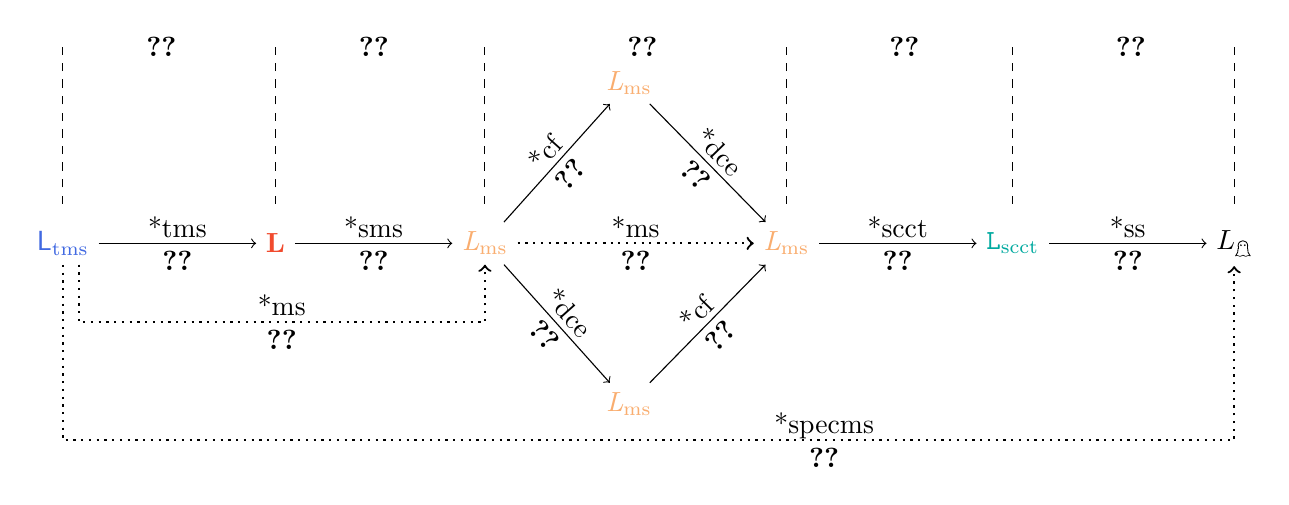
\begin{tikzpicture}
    \node (S) {$\src{L_{\tmssafe}}$};
    \node[right=2.0 of S] (T) {$\trg{L}$};
    \node[right=2.0 of T] (M) {$\irl{L_{\mssafe}}$};
    \node[below right=1.5 and 1.0 of M] (D0) {$\irl{L_{\mssafe}}$};
    \node[above right=1.5 and 1.0 of M] (C0) {$\irl{L_{\mssafe}}$};
    \node[right=3.0 of M] (E) {$\irl{L_{\mssafe}}$};
    \node[right=2.0 of E] (O) {$\obj{L_{\scctsafe}}$};
    \node[right=2.0 of O] (Z) {$\ird{L_{\mathghost}}$};

    \draw[->] (S) to[sloped] node[align=center] (tmsedge) {\gls*{tms}\\ \Cref{thm:cca:rtp:tms}} (T);
    \draw[->] (T) to[sloped] node[align=center] {\gls*{sms}\\ \Cref{thm:ccb:rtp:sms}} (M);
    \draw[->] (M) to[sloped] node[align=center] {\gls*{dce}\\ \Cref{thm:ccdce:rtp:ms}} (D0);
    \draw[->] (M) to[sloped] node[align=center] {\gls*{cf}\\ \Cref{thm:cccf:rtp:ms}} (C0);
    \draw[->] (D0) to[sloped] node[align=center] {\gls*{cf}\\ \Cref{thm:cccf:rtp:ms}} (E);
    \draw[->] (C0) to[sloped] node[align=center] {\gls*{dce}\\ \Cref{thm:ccdce:rtp:ms}} (E);
    \draw[->] (E) to[sloped] node[align=center] {\gls*{scct}\\ \Cref{thm:ccscct:rtp:scct}} (O);
    \draw[->] (O) to[sloped] node[align=center] {\gls*{ss}\\ \Cref{thm:ccspec:rtp:spec}} (Z);

    % Sections
    \node (sectms) at ($(S)+(1.25,2.5)$) {{\Cref{subsec:cs:tms}}};
    \node (secsms) at ($(T)+(1.25,2.5)$) {{\Cref{subsec:cs:ms}}};
    \node (secopts) at ($(M)+(2.0,2.5)$) {{\Cref{subsec:cs:opts}}};
    \node (secscct) at ($(E)+(1.5,2.5)$) {{\Cref{subsec:cs:scct}}};
    \node (secss) at ($(O)+(1.5,2.5)$) {{\Cref{subsec:cs:ss}}};

    \draw[thick,dotted,->] ($(S) + (0.2,-0.27)$) to ($(S) - (-0.2,1)$) to node[align=center] {\gls*{ms}\\ \Cref{corr:ccab:rtp:ms}} ($(M) - (0.0,1)$) to (M);

    \draw[thick,dotted,->] (S) to ($(S) - (0.0,2.5)$) to node[align=center,pos=.65] {\gls*{specms}\\ \Cref{thm:ccall:rtp:specms}} ($(Z) - (0.0,2.5)$) to (Z);

    % \draw[thick,dotted,->] (S) to[bend right=33,sloped] node[align=center] {\gls*{ms}\\ \Cref{corr:ccab:rtp:ms}} (M);
    \draw[thick,dotted,->] (M) to[bend right=0,sloped] node[align=center] {\gls*{ms}\\ \Cref{thm:cccfccdce:rtp:ms}} (E);
%    \draw[thick,dotted,->] (S) to[out=-45,in=198,sloped] node[align=center] {\gls*{ms}+\gls*{scct}\\ \Cref{thm:ccall:rtp:msscct}} (O);
    % \draw[thick,dotted,->] (S) to[out=-40,in=210,sloped] node[align=center,pos=.8] {\gls*{specms}\\ \Cref{thm:ccall:rtp:specms}} (Z);

    \draw[dashed] ($(S)-(0.0,-0.5)$) -- ($(S)-(0.0,-2.5)$);
    \draw[dashed] ($(T)-(0.0,-0.5)$) -- ($(T)-(0.0,-2.5)$);
    \draw[dashed] ($(M)-(0.0,-0.5)$) -- ($(M)-(0.0,-2.5)$);
    \draw[dashed] ($(E)-(0.0,-0.5)$) -- ($(E)-(0.0,-2.5)$);
    \draw[dashed] ($(O)-(0.0,-0.5)$) -- ($(O)-(0.0,-2.5)$);
    \draw[dashed] ($(Z)-(0.0,-0.5)$) -- ($(Z)-(0.0,-2.5)$);
  \end{tikzpicture}
  \vspace{-1em}
  \caption{Visualisation of the optimising compilation pipeline that preserves \gls*{specms}. %
    Vertices in the graph are the programming languages from earlier sections (\Cref{sec:casestud:defs}). %
    Full edges are secure compilers passes.
    Dotted edges are composition of passes and use the presented framework (\Cref{sec:sequential}) to indicate the property they preserve. %
    The dashed lines partition the graph into the sections where the respective theorems are presented.
  }\label{fig:pipeline}
\end{figure*}
The section demonstrates the power of the framework (\Cref{sec:sequential}) by composing these compilers for a secure and optimising compilation chain that robustly preserves \gls*{specms}.
The first step in this chain is the compiler from $\src{L_{\tmssafe}}$ to $\trg{L}$ that robustly preserves just \gls*{tms} (\Cref{thm:cca:rtp:tms}).
From here, another pass from $\trg{L}$ to $\irl{L_{\mssafe}}$ ensures that no out-of-bounds accesses can happen and, thus, programs at this point attain \gls*{sms} (\Cref{thm:ccb:rtp:sms}).
Since these properties compose into \gls*{ms}, composing these passes yields a compiler that robustly preserves \gls*{ms} (\Cref{corr:ccab:rtp:ms}).
Then, the section presents two optimisation passes, namely \gls*{cf} and \gls*{dce}, each of which robustly preserves \gls*{ms} (\Cref{thm:ccdce:rtp:ms,thm:cccf:rtp:ms}).
These passes can be freely ordered in the compilation chain without compromising memory safety (\Cref{thm:cccfccdce:rtp:ms}).
The next step in the chain ensures that code stays \gls*{scct} (\Cref{thm:ccscct:rtp:scct}) when compiled from $\Lms$ to $\Lscct$, which is done by switching on a constant-time mode for the computation.
Lastly, by introducing barriers immediately after branches, speculative leaks via SPECTRE-PHT are prevented when compiling $\Lscct$ to $\Lspec$.
The final result is that the whole compilation chain robustly preserves \gls*{specms} (\Cref{thm:ccall:rtp:specms}).


\subsection{Robust Temporal Memory Safety Preservation}\label{subsec:cs:tms}

The secure compiler from $\Ltms$ to $\Ltrg$ needs to ensure that when execution switches from context to component, the type signatures are respected.
Thus, the compiler inserts the following dynamic typechecks before entering the body of a component-defined function (anything elided is a trivial identity function from source to target):

\vspace{-1em}
{
\begin{gather}
  \begin{align*}%{rcl}
    %\cca(\src{x}) = &\ \trg{x} 
    % \\
  	%&
  	%\qquad
    %\cca(\src{\lbinop{\expr[_{1}]}{\expr[_{2}]}}) = &\ \lbinop[\trg]{\left[\cca(\src{\expr[_{1}]})\right]}{\left[\cca(\src{\expr[_{2}]})\right]} \\
    %\cca(\src{n}) = &\ \trg{n} 
    % \\
    %&
    \cca(\src{\lget{x}{\expr}}) = &\ \lget[\trg]{\trg{x}}{\left[\cca(\src{\expr})\right]} \\
    \cca(\src{\ldelete{x}}) = &\ \ldelete[\trg]{\left[\cca(\src{x})\right]} 
    \\
    \cca(\src{\lfunction{g}{x:\natt\to\type[_{e}]}{\expr}})  =&
  \end{align*}
  \\
  \begin{align*}
%    \cca(\src{\lset{x}{\expr[_{1}]}{\expr[_{2}]}}) & = \lset[\trg]{\left[\cca(\src{x})\right]}{\left[\cca(\src{\expr[_{1}]})\right]}{\left[\cca(\src{\expr_{2}})\right]} \\
% \\ 
\lfunction[\trg]{\trg{g}}{\trg{x}}{\lifz[\trg]{\trg{\lhast{x}{\natt}}}{
                                                            \left[\cca(\src{\expr})\right] %
                                                                                                 }{\labort[\trg]}}
  \end{align*}
\end{gather}
}

\noindent Since $\trg{L}$ has no static typing, an attacker $\trg{\library_{\ctx}}$ can invoke a component function accepting a $\src{\natt}$ with $\trg{\lpair{17}{29}}$.
With the dynamic check, the compiler ensures that execution aborts in such cases.
%The compiler does not insert other checks and proceeds as the identity function (which in this paper amounts to a simple re-colouring of $\src{L_{\tmssafe}}$ to $\trg{L}$ expressions).

Compiling the \texttt{strncpy} function from \Cref{sec:introduction} with $\cca$, the compiler would in this case ensure that the arguments that are evaluated in the compiled \texttt{strncpy} are valid.
%This effectively has no influence on the resulting trace, so a corresponding cross-language trace relation $\sim^{\Ltms}_{\Ltrg}$ is just equality.

$\cca$ is robustly preserving (\Cref{def:rtp}) \gls*{tms}:
\begin{theorem}[$\cca$ secure w.r.t. \gls*{tms}]\label{thm:cca:rtp:tms}
    $\rtp{\cca}{\tmssafe}$ % \Coqed
\end{theorem}

\subsection{Robust Spatial Memory Safety Preservation}\label{subsec:cs:ms}

The spatial memory safety preserving compiler from $\Ltrg$ to $\Lms$ only inserts bounds-checks whenever reading from or writing to memory in order to enforce \gls*{sms}.
These bounds checks need the bounds information, which the compiler keeps around by introducing a fresh identifier $\irl{x_{SIZE}}$ for each allocation that binds $\irl{x}$.
Then, it is simply a matter of referring to that variable and ensuring that memory accesses are in the interval $[\irl{0},\irl{x_{SIZE}})$.
When the check fails, the code aborts.

\begin{nscenter}
% \small
  $$
  \begin{array}{rcl}
    \ccb(\trg{\lnew{x}{\expr[_{1}]}{\expr[_{2}]}}) & = 
                                                   & \llet[\irl]{\irl{x_{SIZE}}}{\ccb(\trg{\expr[_{1}]})}{}
    		\\&&
    		\lnew[\irl]{\irl{x}}{\irl{x_{SIZE}}}{\ccb(\trg{\expr[_{2}]})}
    		 \\
  \ccb(\trg{\lget{x}{\expr}}) & = 
                              & \llet[\irl]{\irl{x_{n}}}{\ccb(\trg{\expr})}{}
  	\\&&
  \lifz[\irl]{\irl{0\le x_{n}<x_{SIZE}}}{\\&&\irl{\lget{x}{x_{n}}}}{}
  		\irl{\labort}
  	  \\
  \ccb(\trg{\lset{x}{\expr[_{1}]}{\expr[_{2}]}}) & = 
                                                 & \llet[\irl]{\irl{x_{n}}}{\ccb(\trg{\expr[_{1}]})}{}
  		\\&&
  \lifz[\irl]{\irl{0\le x_{n}<x_{SIZE}}}{\\&&\lset[\irl]{\irl{x}}{\irl{x_{n}}}{}
  		\ccb(\trg{\expr[_{2}]})
  		}{\irl{\labort}} 
  		% \\
  \end{array}
  $$
\end{nscenter}

\begin{exampleenv}[Instrumented \texttt{strncpy}]
  Consider again \texttt{strncpy}, but instrumented for \gls*{sms}:
    \begin{lstlisting}[language=c,basicstyle=\ttfamily, morekeywords={size_t}]
void strncpy(size_t n, size_t dst_size, char *dst,
             size_t src_size, char *src) {
  for(size_t i = 0; i < src_size
      && src[i] != '\0' && i < n; ++i) {
    if(i < src_size && i < dst_size) {
      dst[i] = src[i];
    }
  }
}
    \end{lstlisting}
Consider context \texttt{strncpy(2, x, y)}, where \texttt{x} and \texttt{y} are pointers to valid regions of memory with allocated space for exactly two cells and do not contain the null-terminating character \texttt{'\textbackslash 0'}.
% 
Without the \gls*{sms} pass, the event $\ev{Use}\ \loc_{x}\ 2;\comp;\unlock$ would appear on the trace, but that indicates an out-of-bounds access! 
Fortunately, with \gls*{sms} mitigation in place, that event does not appear during execution, since the bounds check prevents the condition \texttt{src[i] != '\textbackslash 0'} from executing.
\end{exampleenv}

Contrary to the previous compiler, $\ccb$ may change the trace of the original $\Ltrg$ program: if there is a memory access, it needs to be protected with a bounds check.
% 
The corresponding relation $\sim^{\Ltrg}_{\Lms} : \trg{\trace}\times\irl{\trace}$ that describes this semantic effect of the compiler is defined partially below.
% 
We omit action $\trg{Set}$, which is treated analogously, and any other event, which is related to its cross-language equivalent.
% \footnote{Up to colours.}
% \footnote{In the interest of space, the full details are in the technical report.}

{
\[
  \typerulenolabel{xrel:sms:read}{\trg{n}\text{ in bounds}}{\trg{Get\ \loc\ n;\comp}\sim^{\Ltrg}_{\Lms}\irl{Get\ \loc\ n;\comp}}
\]
% \[
%   \typerulenolabel{xrel:sms:panic}{\trg{n}\text{ out of bounds}}{\trg{Get\ \loc\ n;\comp}\sim^{\Ltrg}_{\Lms}\irl{\lightning}}
% \]
}

% Note that neither $\Ltrg$ nor $\Lms$ expose branches on the trace.\MP{so what?}
For simplicity, we elide the environment that this relation carries around in order to bind each location to its metadata (such as its size), and resolve the ``$\trg{n}$ in/out of bounds'' premise.
% The bounds check mentioned in the premises of the rules above is left abstract for the sake of simplicity, the interested reader can find
% since the precise definition needs some technicalities that only inhibit readability without any technical insights.
% 
We can now prove that compiler $\ccb$ robustly preserves \gls*{sms}.
\begin{theorem}[$\ccb$ secure w.r.t. \gls*{sms}]\label{thm:ccb:rtp:sms}
  $\rtpsim{\ccb}{\smssafe}{\sim^{\Ltrg}_{\Lms}}$ % \Coqed
\end{theorem}

At this point we can compose $\ccb$ with the previous compiler ($\cca$), but in order to do so, we need a trace relation from $\Ltms$ to $\Lms$.
% 
We can obtain this relation by composing the trace relation we just defined ($\sim^{\Ltrg}_{\Lms}$) with the one used by the previous compiler: $\sim^{\Ltms}_{\Ltrg} : \src{\trace}\times\trg{\trace}$.
% 
The latter has not been previously defined (nor has it been used in the related theorem) because that is just an equality relation, since the trace models of $\Ltms$ and of $\Ltrg$ are the same.
% 
Thus, we formally define $\sim^{\Ltms}_{\Lms}: \src{\trace} \times \irl{\trace}$ as the following composition: $\sim^{\Ltms}_{\Ltrg}\bullet\sim^{\Ltrg}_{\Lms}$.
% 
With this relation, \Cref{corr:ccab:rtp:ms} states that the composition of $\cca$ and $\ccb$ is secure w.r.t. \gls*{ms} and it follows from \Cref{thm:cca:rtp:tms,thm:ccb:rtp:sms} using \Cref{thm:rtpsim:sig}.
% 
\begin{corollary}[$\cca\circ\ccb$ secure w.r.t. \gls*{ms}]\label{corr:ccab:rtp:ms}
  $\;$ 

  \begin{nscenter}
    $\rtpsim{\cca\circ\ccb}{\mssafe}{\sim^{\Ltms}_{\Lms}}$ % \Coqed
  \end{nscenter}
\end{corollary}
% 
This proof requires another precondition besides \Cref{thm:ccb:rtp:sms,thm:cca:rtp:tms}: $\sim^{\Ltms}_{\Ltrg}$ needs to be well-formed with respect to $\smssafe$.
This follows trivially since $\sim^{\Ltms}_{\Ltrg}$ is an equality. 
% 
\begin{lemma}[$\sim^{\Ltms}_{\Ltrg}$ well-formed w.r.t. $\smssafe$]\label{lem:wf:ltmsltrg}
$\;$ 

  \begin{nscenter}
  $\wfcsig{\sim^{\Ltms}_{\Ltrg}}{\smssafe}$
  \end{nscenter}
\end{lemma}

\subsection{Optimising Compilers}\label{subsec:cs:opts} 

This section defines two optimising compiler passes from $\Lms$ to $\Lms$ which perform \gls*{dce} and \gls*{cf}, respectively.
The \gls*{dce} pass applies a na\"ive rewrite rule on conditionals.
The \gls*{cf} pass relies on an auxiliary function \texttt{mix} that uses a substitutions accumulator $\irl{\substlist}$ in order to rewrite constant binary operations, e.g., $\irl{{17}-1}$ to $\irl{16}$, and replace variables that are assigned to constants, e.g., $\irl{\llet{x}{7}{x}}$ to $\irl{7}$.

\vspace{-1em}
\begin{gather*}
  \begin{align*}
    \ccdce(\irl{\lifz{true}{\expr[_{1}]}{\expr[_{2}]}}) & = \ccdce(\irl{\expr[_{1}]}) &\\
    \ccdce(\irl{\lifz{false}{\expr[_{1}]}{\expr[_{2}]}}) & = \ccdce(\irl{\expr[_{2}]}) &
  \end{align*}
  \\
  % \begin{align*}
  %   \ccdce(\irl{\lbinop{\expr[_{1}]}{\expr[_{2}]}}) & = \lbinop[\irl]{\ccdce(\irl{\expr[_{1}]})}{\ccdce(\irl{\expr[_{2}]})} &
  % \end{align*}
  % \\[0.25cm]
  \begin{align*}
    \cccf(\irl{\expr}) & = \partialeval{\irl{\expr}}{\irl{\hole{\cdot}}} &
  \end{align*}
  \\[0.125cm]
  \begin{align*}
   \partialeval{\irl{x}}{\irl{\substlist}} & = \irl{n} 
   	\qquad\qquad \text{if } \irl{\subst{n}{x}}\in\irl{\substlist} \\
   \partialeval{\irl{x}}{\irl{\substlist}} & = \irl{x} 
   \qquad\qquad \text{if } \irl{\subst{n}{x}}\notin\irl{\substlist} \\
   \partialeval{\irl{\lbinop{n}{m}}}{\irl{\substlist}} & = \irl{k} 
   \qquad\qquad \text{if } \lbinop{\irl{n}}{\irl{m}}=k \\
   %\partialeval{\irl{\lbinop{\expr[_{1}]}{\expr[_{2}]}}}{\irl{\substlist}} & = \lbinop[\irl]{\partialeval{\irl{\expr[_{1}]}}{\irl{\substlist}}}{\partialeval{\irl{\expr[_{2}]}}{\irl{\substlist}}} \\
   \partialeval{\irl{\llet{x}{n}{\expr}}}{\irl{\substlist}} & = \partialeval{\irl{\expr}}{\irl{\subst{n}{x}\cdot\substlist}} 
  % \\
  % \partialeval{\irl{\lget{x}{\expr}}}{\irl{\substlist}} & = \lget[\irl]{\irl{x}}{\partialeval{\irl{\expr}}{\irl{\substlist}}}
% \end{align*}
\end{align*}
% \\
% \begin{align*}
%   \partialeval{\irl{\llet{x}{\expr[_{1}]}{\expr[_{2}]}}}{\irl{\substlist}} & = \llet[\irl]{\irl{x}}{\partialeval{\irl{\expr[_{1}]}}{\irl{\substlist}}}{\\&\partialeval{\irl{\expr[_{2}]}}{\irl{\substlist}}} \\
%   \partialeval{\irl{\lifz{\expr[_{1}]}{\expr[_{2}]}{\expr[_{3}]}}}{\irl{\substlist}} & = \lifz[\irl]{\partialeval{\irl{\expr[_{1}]}}{\irl{\substlist}}}{\\&\partialeval{\irl{\expr[_{2}]}}{\irl{\substlist}}}{\partialeval{\irl{\expr[_{3}]}}{\irl{\substlist}}} \\
% \end{align*}
\end{gather*}
% \vspace{-3em}

Note that both passes have no effect on the resulting trace of a program, up to $\emptyevent$-steps. 
Because of this, both passes have equality as corresponding cross language trace relation. 
Moreover, it is straightforward to prove both passes as secure (\Cref{def:rtp}) w.r.t. \gls*{ms}. 

\begin{theorem}[$\ccdce$ secure w.r.t. \gls*{ms}]\label{thm:ccdce:rtp:ms}
  $\rtp{\ccdce}{\mssafe}$ %\Coqed
\end{theorem}
\begin{theorem}[$\cccf$ secure w.r.t. \gls*{ms}]\label{thm:cccf:rtp:ms}
  $\rtp{\cccf}{\mssafe}$ %\Coqe
\end{theorem}

With both \Cref{thm:ccdce:rtp:ms,thm:cccf:rtp:ms} it follows from \Cref{corr:swappable} that the two passes can be interchanged arbitrarily:

\begin{theorem}[$\cccf\circ\ccdce$ and $\cccf\circ\ccdce$ are secure w.r.t. \gls*{ms}]\label{thm:cccfccdce:rtp:ms}
$\;$ 

  \begin{nscenter}
  \phantom{and~}\!\!$\rtp{\cccf\circ\ccdce}{\mssafe}$ 

  and~$\rtp{\ccdce\circ\cccf}{\mssafe}$ % \Coqed
  \end{nscenter}
\end{theorem}

\subsection{Robust Strict Cryptographic Constant Time Preservation}\label{subsec:cs:scct}

This section defines a compiler $\ccscct$ from $\Lms$ to $\Lscct$ that robustly preserves \gls*{scct}. 
Given the fact that $\Lscct$ provides a \gls*{cct}-mode that can be turned on or off, the compiler inserts wrapper code for function calls and function bodies to ensure that execution in the component always happen in \gls*{cct}-mode.
This simple flag combines the effect of FaCT~\cite{cauligi2019fact} 

\vspace{-1em}
\[
\begin{array}{rcl}
  \ccscct(\irl{\lfunction{g}{x}{\expr}}) & = & \lfunction[\obj]{\obj{g}}{\obj{x}}{\obj{\lwrdoit{ON};}\ccscct(\irl{\expr})} \\
  \ccscct(\irl{\lcall{g}{\expr}}) & = & \lcall[\obj]{\obj{g}}{\ccscct(\irl{\expr})\obj{; \lwrdoit{ON}}} 
    % \\
    % \ccscct(\irl{\lbinop{\expr[_{1}]}{\expr[_{2}]}}) & = \lbinop[\obj]{\ccscct{\irl{\expr[_{1}]}}}{\ccscct{\irl{\expr[_{2}]}}} 
    % \\
\end{array}
\]
% \vspace{-2em}
%
The context can overwrite the flag and exit the mode, but upon invoking a function that is part of the component, the flag is set again.
Because of this, the corresponding cross-language trace relation $\sim^{\Lms}_{\Lscct}$, only relates events without secrets:%

\begin{center} 
  \typerulenolabel{xrel:scct:noleak}{}{\irl{\preevent;\comp}\sim^{\Lms}_{\Lscct}\obj{\preevent;\comp;\unlock}}
\end{center}

The compiler is secure w.r.t. \gls*{scct}: %, similarly proven as in \Cref{subsec:cs:tms}.

\begin{theorem}[$\ccscct$ secure w.r.t. \gls*{scct}]\label{thm:ccscct:rtp:scct}
  \small
  $\rtpsim{\ccscct}{\scctsafe}{\sim^{\Lms}_{\Lscct}}$ % \Coqed
\end{theorem}

\subsection{Robust Speculative Safety Preservation}\label{subsec:cs:ss}

This section defines the final compilation pass $\ccspec$, which ensures that $\Lscct$ programs, which are assumed to be \gls*{ss}, stay \gls*{ss} at $\Lspec$-level. 
To do so, $\ccspec$ inserts a speculation barrier after branches, which is sufficient to harden the program against speculative leaks, since SPECTRE-PHT~\cite{kocher2019spectre} is the only speculative leak modeled in the semantics of $\Lspec$.

\vspace{-1em}
\[
\begin{array}{cl}
  &\ccspec{(\obj{\lifz{\expr[_0]}{\expr[_1]}{\expr[_2]}})} = 
  \\
  &\qquad\qquad \lifz[\ird]{\ccspec{\left(\obj{\expr[_0]}\right)}}{\ird{\lbarrier;}\ccspec{\left(\obj{\expr[_1]}\right)} \\&\qquad\qquad}{ \ird{\lbarrier;}\ccspec{\left(\obj{\expr[_2]}\right)}} 
\end{array}
\]
% \vspace{-2em}
%

Clearly, the corresponding cross-language trace relation $\sim^{\Lscct}_{\Lspec}$ has only one non-trivial case: for branches, only relate them where speculation is blocked by a barrier:

\begin{center}
  \typerulenolabel{xrel:spec:if}{}{\obj{Branch\ n}\sim^{\Lscct}_{\Lspec}\ird{Branch\ n}\cdot\ird{Spec}\cdot\ird{Barrier}\cdot\ird{Rlb}}
\end{center}

The base-event relation above scales to full events by ensuring the missing annotations ($\obj{\comp;\securitytag{}}$ and $\ird{\comp;\securitytag{}}$) are the same.
% 
With this relation, we prove that $\ccspec$ is secure with respect to \gls*{ss}.
\begin{theorem}[$\ccspec$ secure w.r.t. \gls*{ss}]\label{thm:ccspec:rtp:spec}
  \small$\rtpsim{\ccspec}{\sssafe}{\sim^{\Lscct}_{\Lspec}}$ % \Coqed
\end{theorem}

\subsection{Robust Preservation of Memory Safety, Strict Cryptographic Constant Time, and Speculative Safety}

Finally, this subsection combines all previous results into one compilation chain to get that it preserves full \gls*{specms}.
Let $\ccspecms$ be the compiler that is the composition of $\cca$, $\ccb$, $\cccf$, $\ccdce$, $\ccscct$, and $\ccspec$. 
Let $\sim^{\Ltms}_{\Lspec}$ be the composition of $\sim^{\Ltms}_{\Lms}$, $\sim^{\Lms}_{\Lscct}$, and $\sim^{\Lscct}_{\Lspec}$.
Then, the following corollary holds.

\begin{corollary}[$\ccspecms$ secure w.r.t. \gls*{specms}]\label{thm:ccall:rtp:specms}
  $\;$ 

  \begin{nscenter}
    $\rtpsim{\cc{\Ltms}{\Lspec}}{\mssafe\cap\scctsafe\cap\sssafe}{\sim^{\Ltms}_{\Lspec}}$ % \Coqed
  \end{nscenter}
\end{corollary}

As with \Cref{corr:ccab:rtp:ms}, it is important to ensure that the respective cross language trace relations are well-formed (\Cref{def:wfc:sig:tracerel}).
It is already known that $\sim^{\Ltms}_{\Lms}$ is well-formed with respect to $\mssafe$ (\Cref{lem:wf:ltmsltrg}).
Next in the chain is $\sim^{\Lms}_{\Lscct}$, which has to be well-formed w.r.t. $\scctsafe$.
This lemma holds, since a trace that was $\scctsafe$ is $\scctsafe$ even after applying $\sim^{\Lms}_{\Lscct}$: the relation enforces that $\Lscct$ traces related to $\Lms$ traces have no leaks of secrets whatsoever.

\begin{lemma}[$\sim^{\Lms}_{\Lscct}$ well-formed w.r.t. $\scctsafe$]\label{lem:wf:lsmslscct}
$\;$ 

  \begin{nscenter}
  $\wfcsig{\sim^{\Lms}_{\Lscct}}{\scctsafe}$
  \end{nscenter}
\end{lemma}

The last relation is $\sim^{\Lscct}_{\Lspec}$ which needs to be well-formed w.r.t. $\sssafe$.
Similarly to the previous relation, this holds, since $\sim^{\Lscct}_{\Lspec}$ only relates $\Lspec$ traces, which do not have speculative leaks, with $\Lscct$ traces.

\begin{lemma}[$\sim^{\Lscct}_{\Lspec}$ well-formed w.r.t. $\sssafe$]\label{lem:wf:lscctlspec}
  $\wfcsig{\sim^{\Lscct}_{\Lspec}}{\sssafe}$
\end{lemma}












\section{Formal Insights}\label{sec:formalities}

This section discusses how to connect each language-specific security property to the general security properties of \Cref{sec:compprop} (\Cref{subsec:formalities:maps}), and it demonstrates that the security property resulting from the universal image projection is faithful to the original property (\Cref{subsec:formalities:props}). 
% 
Then, this section discusses why the order of compiler passes matters, and how does our framework help with identifying insecure compositions (\Cref{subsec:compatsecpasses}), and it gives additional technical insights on the secure compilation proofs (\Cref{subsec:seccompproofs}).

\subsection{From Language Traces to General Ones}\label{subsec:formalities:maps}

The previous theorems talk about preserving properties expressed in the trace model of the languages of each compiler.
However, these trace models are not the same trace model we used to specify the properties of \Cref{sec:compprop} (indicated with \ev{L}), which serves as the ``ground truth'' for the meaning of our properties.
% 
To bridge this gap, the formal development requires specifying additional trace relations, from each of the language trace models to the \ev{L} one, that, for example, relate $\src{Get\ \loc\ n}$ and $\src{Set\ \loc\ n}$ to $\ev{Use\ \loc\ n}$ (and that induce a related universal image that we use in \Cref{subsec:formalities:props}).
% 
One key insight of these relations is that they all omit context-made actions for two reasons: (1) contexts (which are universally quantified) can trivially invalidate any property and (2) we are interested in the component upholding the properties.
% 

 % disregarded a glaring but minor technical issue: take $\tmssafe$ (\Cref{def:trace:tmsdef}) as an example.
% It contains traces as specified in \Cref{subsec:basic:memsafety:tracemodel}.
% However, these are different from $\Ltms$ traces (\Cref{subsec:ltms}) which means that \Cref{thm:wt:tms} is ``ill-typed''.
% Similarly for the other theorems.
% In the interest of reducing visual baggage, the notation left out yet another cross-language trace relation, translating language-specific traces into these non-language specific traces. 
% In doing so, context-level actions are dropped and, e.g., both $\src{Get\ \loc\ n}$ and $\src{Set\ \loc\ n}$ are translated into $\ev{Use\ \loc\ n}$.


\subsection{Security Properties and Their Meaning}\label{subsec:formalities:props}
Each of the presented compilers uses a cross-language trace relation, which is also used to translate the property from one language to the other one (via the existential or universal images).
% 
%Whenever such translations occur, it is important to check whether there has been a change of meaning.
%Secure compiler engineers need to ensure that such translations of properties do not change meaning in a fundamental wrong way. 
% lifting or lowering reasoning from target- to source-level or vice-versa,
While the meaning of projected properties does change with a translation, the change should not allow for a flawed compilation pipeline.
% 
For example, we could be using a trace relation that translates a property in a language to a totally different one in another language.
% 
To raise the trust into the translation of properties, \Cref{thm:prop-rel-corr} states (in a general fashion) that each security property is faithfully translated using the universal image according to the cross-language trace relation induced by the compiler.

\begin{theorem}[Properties Relation Correctness]\label{thm:prop-rel-corr}
  \begin{align*}
    \forall& \pi \in \{\tmssafe,\smssafe,\scctsafe,\sssafe\}, 
    \\
    \text{ for each }& \text{pair of languages } \src{L} \text{ and } \trg{L} \text{ used by the compilers},
    \\
    \text{ if }& 
    % \tau_{\sim^{\trg{L}}_{\ev{L}}}(\pi) \sim^{\trg{L}}_{\ev{L}} \pi
    \sigma_{\sim^{\trg{L}}_{\ev{L}}}(\pi) \sim^{\trg{L}}_{\ev{L}} \pi
    \text{ and } 
    % \sigma_{\sim^{\src{L}}_{\trg{L}}}(\tau_{\sim^{\trg{L}}_{\ev{L}}}(\pi)) \sim^{\src{L}}_{\trg{L}} \tau_{\sim^{\trg{L}}_{\ev{L}}}(\pi)
    \sigma_{\sim^{\src{L}}_{\trg{L}}}(\sigma_{\sim^{\trg{L}}_{\ev{L}}}(\pi)) \sim^{\src{L}}_{\trg{L}} \sigma_{\sim^{\trg{L}}_{\ev{L}}}(\pi)
    \\
    \text{ then }& 
    % \tau_{\sim^{\src{L}}_{\ev{L}}}(\pi) = \sigma_{\sim^{\src{L}}_{\trg{L}}}(\tau_{\sim^{\trg{L}}_{\ev{L}}}(\pi)) 
    \sigma_{\sim^{\src{L}}_{\trg{L}}}(\sigma_{\sim^{\trg{L}}_{\ev{L}}}(\pi)) \sim^{\src{L}}_{\ev{L}} \pi
  \end{align*}
\end{theorem}
The complexity of this theorem is that the relation in the conclusion cannot be obtained by composing the two relations in the premises.
% 
%% MK: the following does not say anything about the theorem, only about the syntactic compiler
%What happens in practice is that compiler engineers are given the relations from each language to \ev{L} and they need to build a compiler that induces a relation $\sim^{\src{L}}_{\trg{L}}$ that respects this theorem.
% 

We now informally argue why this theorem holds for the composition of all considered properties from \Cref{sec:compprop}.

\paragraph{$\sigma_{\sim^{\Ltms}_{\Lms}}\left(\tmssafe\cap\smssafe\cap\scctsafe\cap\sssafe\right)$}

For the four properties considered here, the trace models of $\Ltms$, $\Ltrg$, and $\Lms$ do not consider actions related to $\scctsafe$ and $\sssafe$, so these two properties are trivially translated correctly.
% 
We now discuss the remaining $\tmssafe$ and $\smssafe$ in the form of their intersection $\mssafe$.

Recall that $\sim^{\Ltms}_{\Lms}$ is the composition of $\sim^{\Ltms}_{\Ltrg}$ and $\sim^{\Ltms}_{\Lms}$.
% 
Since $\sim^{\Ltms}_{\Ltrg}$ is an equality, this relation trivially preserves the meaning of translated properties: related traces are identical!

Finally, let us consider a trace $\irl{\trace}\in\mssafe$ and understand what is related to via $\sim^{\Ltrg}_{\Lms}$.
% 
{\em All} traces $\trg{\trace}$ with $\trg{\trace}\sim^{\Ltrg}_{\Lms}\irl{\trace}$ are identical to $\irl{\trace}$ except for get and set actions, which require for in-bound accesses (as stated in \Cref{subsec:cs:ms}): this clearly respect $\mssafe$.
% 

% In both cases, the translated event does not represent an out-of-bounds memory access. 

% \footnote{Both $\sim^{\Ltms}_{\Ltrg}$ and $\sim^{\Ltrg}_{\Lms}$ filter context actions.}.

% Now, starting from $\mssafe$ expressed in $\Lms$, we check that its translation in $\Ltms$ is still $\mssafe$.
% % 
% We can see that the property resulting from the projection of $\Lms$ traces back to $\Ltms$ faithfully models $\mssafe$, which translates to both $\scctsafe$ and $\sssafe$, 
% \MPin{ equiv  +  other rel only adds traces that fail }
% since these properties trivially hold for $\Ltms$, $\Ltrg$, and $\Lms$ traces.


\paragraph{$\sigma_{\sim^{\Lms}_{\Lscct}}\left(\tmssafe\cap\smssafe\cap\scctsafe\cap\sssafe\right)$}

As before, the trace models of $\Lscct$ and $\Lms$ cannot express $\sssafe$, so that is trivially translated correctly.
% 
Also, the trace model of $\Lscct$ extends the one of $\Lms$ with respect to $\tmssafe$ and $\smssafe$ events, so the translation argument regarding those two properties is the same as before.
% 
Thus, we need to reason about whether $\scctsafe$ is translated correctly.

By definition, $\sim^{\Lms}_{\Lscct}$ only relates $\obj{\unlock}$ events, which is also the same relation induced by $\sim_{\ctsafe}$ in \Cref{sec:msscct-rel}.
% 
This ensures that composing the relations only relates $\unlock$ events, and thus the property is translated correctly.

% Consider a trace $\obj{\trace}\in\scctsafe$ and all $\irl{\trace}$ such that $\irl{\trace}\sim^{\Lms}_{\Lscct}\obj{\trace}$. 
% In turn, $\obj{\trace}$ cannot contain any leaks of secret values, so it cannot violate $\scctsafe$.
% Toggling data-independent timing mode has no impact on $\mssafe$ or $\sssafe$.

\paragraph{$\sigma_{\sim^{\Lscct}_{\Lspec}}\left(\tmssafe\cap\smssafe\cap\scctsafe\cap\sssafe\right)$}
The trace model of $\Lspec$ extends the one of $\Lscct$ with respect to $\tmssafe$, $\smssafe$, and $\scctsafe$, so the translation argument for those three properties is the same as before.
% 
Concerning $\sssafe$, $\sim^{\Lscct}_{\Lspec}$ relates $\Lspec$ speculation traces with $\Lscct$ branches with the $\lock_{\text{NONE}}$ tag, so the property is translated correctly, according to the relation defined in \Cref{sec:spec-ms-rel}.
 % introducing $\ird{barrier}$ never violates $\sssafe$ and has no effect on $\mssafe$ or $\scctsafe$.

%\MPin{
%	can this be made formal?
%	what's the point?
%}

\subsection{Compatibility of Secure Compiler Passes}\label{subsec:compatsecpasses}

% \Cref{thm:rtpsim:sig} is applicable, up to the well-formedness of $\sim_1$ w.r.t. $\trg{\class[_2]}$.
Consider applying $\ccspec$ first and then $\ccb$ (albeit currently syntactically impossible).
% , let us pretend that it is possible by just extending $\ccb$ for the constructs present in $\Lscct$ that are not present in $\Ltrg$.
% Clearly, as evidenced earlier (\Cref{subsec:formalities:props}), $\ccb\cdot\ccspec$ is an acceptable composition that yields an interesting class of security properties, i.e., $\sigma_{\sim_{\irl{ms}}\bullet\sim_{\ird{\mathghost}}}\left(\mssafe\cap\scctsafe\cap\sssafe\right)$. 
In this case, $\ccb$ would insert new branches into the code that are not protected by a speculation barrier! 
This concern is reflected in the proofs that establish that the security class resulting of the composition of the trace relations is meaningful.
% , much similar to ensuring that a definition models what the formal methods expert intends to model. 
For the $\ccspec\cdot\ccb$ case, the class is $\sigma_{\sim_{\ird{\mathghost}}\bullet\sim_{\irl{ms}}}\left(\mssafe\cap\scctsafe\cap\sssafe\right)$.
Since $\ev{Use\ \loc\ n}\sim_{\irl{ms}}\irl{Branch\ n}\cdot\irl{Spec}\cdots$, where $\cdots$ does not contain a $\ev{{Barrier}}$ event, the resulting class is \emph{not} the original $\sssafe$ that is intended and it would break the corresponding \Cref{thm:prop-rel-corr}.
% Because of this, it is crucial to analyse the precise shape of the class of properties after mapping a target-level property to a source-level property\footnote{Dito for mapping a source-level property to a target-level property.}.

However, the composition is still technically possible and it is the job of the compiler engineers to ensure that the secure compilation pipeline happens in an order that ensures that the mapped security property is the intended one.

\subsection{Secure Compilation Proofs}\label{subsec:seccompproofs}

Our secure compilation proofs rely on backtranslations~\cite{abate2019jour,patrignani2021rsc}, which let one construct a source context starting from either target traces (aka trace-based backtranslations) or target contexts (aka context-based backtranslations).
These backtranslations also require setting up cross-language relations between various language elements such as expressions and program states, so we leave these details for the technical reports.
% , the usual strategy is to establish a backwards simulation between source components and their compiled target counterpart. 
% For the universally quantified target context, a technique known as backtranslation is well-established, which constructs a source-level context either by backtranslating the target-level context, amounting to a ``decompilation'', or by constructing it using the target-level trace, so that the source-context emits parts of the whole execution trace that are related to the parts emitted by the target-level context. 
All backtranslations in the case-study are trace based except for those required by $\ccdce$ and $\cccf$, which are context-based (and they are an identity function). 
% Since these optimisations have no significant semantic effect and source- and target-language are equal, the backtranslation amounts to an identity translation. 

\section{Related Work\pages{2}}\label{sec:relwork}

This section discusses robust compilation, other secure compilation criteria and work related to the properties preserved in the case study.
% (\Cref{subsec:relw:seccomprtp}) 
% (\Cref{subsec:relw:seccompcrit}).
% Since the case study of \Cref{sec:casestud:defs,sec:casestud:rtp} implements measures for preserving \gls*{ms}, \gls*{cct}, and \gls*{ss}, 
% Then, this section discusses work related 
% relevant related work as well 
% (\Cref{subsec:relw:msmechs,subsec:relw:cctmechs,subsec:relw:ssmechs}).

\paragraph*{Secure Compilation as Robust Preservation}\label{subsec:relw:seccomprtp}

The robust preservation of properties as a compiler-level criterion has been analysed extensively~\cite{abate2019jour,patrignani2021rsc,abate2021extacc,patrignani2019survey} and thus we build on that framework.
No existing work is concerned with composing secure compilers, however, existing work~\cite{abate2021extacc} sketches composition of trace-relating compiler correctness in a similar way to what has been presented here.
%Parts of these works consider languages with different trace models and our technical setup can handle this. 
The work relating robust preservation with universal composability~\cite{patrignani2022universal} is closest to what this paper presents.
% 
The authors demonstrate a similar compositionality theorem to ours (\Cref{sec:sequential}) but use it in the context of protocols.
% 
The work does not consider the generality to support different trace models or composition of compilers which robustly preserve different classes.
% The authors demonstrate a similar compositionality theorem to what is presented here (\Cref{sec:sequential}) as well as in an earlier version of this work~\cite{kruse2022csc}.
% However, they do not demonstrate the scalability of the approach by means of a case study.

%\paragraph*{Composition of Secure Compilers}\label{subsec:relw:seccompcomp}

There is work on lifting exploits for single compilers to the whole chain~\cite{paykin2019weird}.
%Our framework does not consider exploits.
%\MP{ a bit dry and short}
While that work considers {\em in}secure compilation and composition thereof in terms of exploits, the composition they are interested in allows to lift an exploit for one compiler pass to the whole compilation chain. 
Our framework takes the opposite direction and provides compositionality results for secure compilers.
%
%
%To the best of our knowledge, there does not exist published work discussing the compositionality of the robust preservation criterion, the gold-standard of secure compilation.

\paragraph*{Other Secure Compilation Criteria}\label{subsec:relw:seccompcrit}

While this paper focuses on the robust preservation framework~\cite{abate2019jour}, other secure compilation criteria exist.
The survey on formal approaches to secure compilation~\cite{patrignani2019survey} discusses a broad spectrum already, while this section presents a very high-level overview.
Fully abstract compilation~\cite{abadi1999fullabstraction} states that a compiler should preserve and reflect observational equivalence between source and target programs.
Abate \emph{et al.}~\cite{abate2021faandrc} showed that fully abstract compilers robustly preserve program properties that are either trivial or meaningless.
As a mitigation for this, the authors presented a categorical approach based on maps of distributive laws~\cite{watanabe2002modl}, which they call many maps of distributive laws.
Maps of distributive laws have been investigated before as a possible secure compilation criterion~\cite{tsampas2020catsc}.
Other approaches are extensions of the compiler correctness criterion as discussed in other work~\cite{patterson2019next700} or the introduction of opaque observations~\cite{vu2021reconciling} to reconcile compiler optimisations with security.
Note that this work also presents secure compilers that are optimising, but contrary to the other~\cite{vu2021reconciling}, provides a formal account of these in the robust preservation framework.
% Lastly, the authors of this paper have presented ongoing work~\cite{patrignani2023blame} on a weaker robust preservation criteria based on the concept blame.

\paragraph*{Memory Safety Mechanisms}\label{subsec:relw:msmechs}

Different mechanisms for enforcing memory safety exist that also consider the secure compilation domain, i.e., have an active attacker model.
For example, the ``pointers as capabilities'' principle represents pointers as machine-level capabilities~\cite{korashy2021capableptrs}, which behave in a similar fashion to capabilities by means of linear typing~\cite{morrisett2005L3}.
The approach of this paper also uses linear typing, but differs from $L^{3}$~\cite{morrisett2005L3} in the way that functions are not first-class.
Moreover, this paper considers an active attacker, while the work on $L^{3}$ only discusses whole programs and, thus, has no active attacker model.
The instrumentation to ensure memory safety that this paper presents is inspired by Softbounds~\cite{nagarakatte2009soft}.
That work inserts bounds-checks in front of pointer-dereferences and, for this to work, inserts meta-data information on pointer creation.
Softbounds also works in a more advanced setting with structured fields accesses and also introduces a table-lookup for pointers that are stored in memory.
This paper only considers arrays of primitive data, i.e., there are no pointers to pointers or structures.
Several other approaches to memory-safety exist in literature, specifically as compiler instrumentations~\cite{akritidis2009baggy,younan2010paricheck,jung2021pico,shankaranarayana2023tailcheck,dhumbumroong2020boundwarden,nam2019framer,zhou2023fatptrs}, hardware-extensions~\cite{kwon2013lowfat,saileshwar2022heapcheck,chen2023flexpointer,kim2023whistle}, or programming language extensions~\cite{elliott2018checkedc,li2022formalcheckedc,jim2002cyclone,elliott2015guilt,west2005cuckoo,weis2019fyr,benoit2019uniqueness}.
What differentiates this work from them is that this work uses known, compiler-based approaches to ensure memory-safety as a means to investigate secure compiler compositions.
This paper does not provide efficient memory-safety, but serves as a theoretical foundation for the secure compilation domain.

To extend the languages in this paper with a less restricted form of pointer arithmetic, the region colouring memory safety monitor presented in earlier work~\cite{michael2023mswasm} can be used.
The work presenting this monitor provides an approach for the robust preservation of memory safety compiling from C to WASM.
However, they do not discuss composition of secure compilers but rather investigate an instance of a secure compiler.

\paragraph*{Cryptographic Constant Time Mechanisms}\label{subsec:relw:cctmechs}

The approach to preserving cryptographic constant time in this paper is high-level, where a programming language exposes a way to switch the semantics to a data (operand) independent timing mode.
Since identifiers in $\Lscct$ are annotated with a secrecy tag, this approach is similar to others with information flow control.
For example, Vale~\cite{bond2017vale} uses Dafny to ensure constant-time assembly code, while Jasmin~\cite{almeida2017jasmin} makes use of the Coq proof assistant to reject non-constant-time programs.
CT-Wasm~\cite{watt2019ctwasm} enforces constant-timeness by means of a type system.
Different to the approach of this paper, these approaches necessitate that the programmer writes \gls*{cct} code.
An approach to allow programmers to write more high-level code is CryptOpt~\cite{kuepper2023cryptopt}, which generates efficient target-code by means of a randomised search.
This paper abstracts over concrete mitigation strategies and simply assumes that there is a flag to switch to a cryptographic-constant time execution mode.
This can be realised by employing the FaCT~\cite{cauligi2019fact} compiler, which translates common non-constant time code patterns to be constant-time, and the data (object) independent timing execution mode of modern processors.

\paragraph*{Speculation Safety Mechanisms}\label{subsec:relw:ssmechs}

This paper uses a taint-tracking mechanism inspired by existing work~\cite{guarnieri2018spectector,fabian2022automatic}.
These taints are used to express absence of any speculative leaks in \gls*{ss}~\cite{guarnieri2018spectector}. 
The semantics of $\Lspec$ hardcodes the kind of speculative leaks to just SPECTRE-PHT~\cite{kocher2019spectre}, but future work could use semantics composition~\cite{fabian2022automatic} to support more variants.
Note that our framework composes compilers and not semantics. 

%This work has taken inspiration in the sematics of $\Lspec$ and in \Cref{def:trace:ss} from recent formalisations~\cite{guarnieri2018spectector,fabian2022automatic}.
% \MPin{
%  we take SS from exorcising.
%  we do not take SNI from spectector because it is a hypersafety.
%  other work defined similar props. 
% }
% A subsequent line of work~\cite{fabian2022automatic} shows how to modularly define and compose formal semantics that models different speculative execution variants. 
% Recent work~\cite{fabian2024lift} demonstrates how to lift existing secure compilation proofs for security properties related to speculative execution to more powerful properties, i.e., properties defined for languages with a trace model that enables more vulnerabilities, such as combinations of different speculative execution exploits. 
% To this end, they define a lifting framework and demonstrate how a secure compilation proof for a weaker property can be lifted to a stronger one. 
% Contrary to the compositionality framework presented in this paper, these works are only concerned with composing semantics of the respective programming languages, while in this paper, the secure compilers themselves are composed.

\section{Conclusion\pages{$\sfrac{1}{2}$}}\label{sec:concl}
This paper tackles the problem of understanding what kind of security properties a secure compiler preserves, when said compiler is the combination of compiler passes that preserve possibly different security properties.
% 
%For this, this paper first formalised security properties of interest and their composition.
% 
The paper proves that composing secure compilers that preserve certain properties results in a secure compiler that preserves the composition of these properties.
% While the presented security property composition relied on monitors that check only trace-properties, the composition of secure compilers does not make any restriction towards the kind of property involved in the composition. 
% It is subject to future work to develop techniques to verify relational hyperproperties~\cite{abate2019jour}, while the composition of hyperproperties could be very similar to the composition of ordinary properties as presented in this paper, since hyperproperties can be checked with an automata-based model-checker~\cite{beutner23hyperltl}.
% 
Finally, this paper defines a multi-pass compiler and proves that it preserves \gls*{specms}.
Crucially, this paper derives the security of the multi-pass compiler from the composition of the security properties preserved by its individual passes, which include security-preserving as well as optimisation passes.
% For future work, it is interesting to look at more sophisticated optimisation passes that, e.g., reorder events that appear on traces.


\newpage

\bibliographystyle{IEEEtranS}
\bibliography{main}

%%
%% If your work has an appendix, this is the place to put it.
\appendix
\subsection{Existential Image}\label{subsec:extimg}

\begin{definition}[Existential Image]
% [Existential and Universal Image]
\label{def:existential:img}\label{def:tau}
  \[
    \tau_\sim\left(\src{\pi}\right) := 
      \left\{ 
        \trg{\trace} \mid \exists \src{\trace}\ldotp \src{\trace}\sim\trg{\trace}, \text{ and } \src{\trace}\in\src{\pi} 
      \right\}
  \]
  %\[ 
  %  \sigma_\sim\left(\trg{\pi}\right) := 
  %    \left\{ 
  %      \src{\trace} \mid \forall \trg{\trace}\ldotp \text{if }\src{\trace}\sim\trg{\trace}, \text{ then } \trg{\trace}\in\trg{\pi} 
  %    \right\}
  %\]
\end{definition}

\begin{definition}[Robust Preservation with $\tau_\sim$]\label{def:rtp:tau}
  % $\;$\\
  % \vspace{-1em}
  % \begin{nscenter}
  % Compiler $\cc{\src{L}}{\trg{L}}$ robustly preserves $\class$, 
  {$\rtptau{\cc{\src{L}}{\trg{L}}}{\src{\class}}{\sim}$}
  %, iff 
  $\isdef$
    {$\forall \src{\pi}\in\src{\class}, \src{p}\in\src{L},$} if {$\rsat{\src{\progvar}}{\src{\pi}}$}, then {$\rsat{\cc{\src{L}}{\trg{L}}\left(\src{p}\right)}{\tau_\sim\left(\src{\pi}\right)}$}.
  % \end{nscenter}
\end{definition}

\begin{theorem}[Composition of Secure Compilers w.r.t. $\tau$]\label{thm:rtpsim:tau}
  $\;$ 

  If {$\rtptau{\cc{\src{L}}{\trg{L}}}{\src{\class[_{1}]}}{\sim_1}$}, {$\rtptau{\cc{\trg{L}}{\obj{L}}}{\tilde{\tau}_{\sim_1}\left(\src{\class[_2]}\right)}{\sim_2}$}, and {$\wfctau{\sim_1}{\src{\class[_2]}}$}, \\ then {$\rtptau{\cc{\src{L}}{\trg{L}}\circ\cc{\trg{L}}{\obj{L}}}{\src{\class[_{1}]}\cap\src{\class[_{2}]}}{\sim_1\bullet\sim_2}$}. \Coqed
\end{theorem}

\begin{corollary}[Swapping Secure Compiler Passes]\label{corr:swappable:tau}
  $\;$ 

  If {$\rtptau{\cc[_{1}]{\trg{L}}{\trg{L}}}{\src{\class[_{1}]}}{\sim_1}$ and $\rtptau{\cc[_{2}]{\trg{L}}{\trg{L}}}{\src{\class[_{2}]}}{\sim_2}$}, %
  {$\wfctau{\sim_1}{\src{\class[_2]}}$ and $\wfctau{\sim_2}{\src{\class[_1]}}$}, %
  and {$\tilde{\tau}_{\sim_1}\left(\src{\class[_2]}\right)=\src{\class[_2]}$ as well as $\tilde{\tau}_{\sim_2}\left(\src{\class[_1]}\right)=\src{\class[_1]}$},
  then {$\rtptau{\cc[_{1}]{\trg{L}}{\trg{L}}\circ\cc[_{2}]{\trg{L}}{\trg{L}}}{\src{\class[_{1}]}\cap\src{\class[_{2}]}}{\sim_1\circ\sim_2}$ and $\rtptau{\cc[_{2}]{\trg{L}}{\trg{L}}\circ\cc[_{1}]{\trg{L}}{\trg{L}}}{\src{\class[_{2}]}\cap\src{\class[_{1}]}}{\sim_2\circ\sim_1}$}. \Coqed
\end{corollary}

\subsection{Secure Upper and Lower Composition}\label{sec:other-compos}
Besides sequential composition, there are two other compositions, namely an {\em upper}, i.e., a compiler that takes multiple inputs and yields one output, and a {\em lower} composition, i.e., a compiler that takes one input and yields multiple outputs.
We {define the upper composition $\cc{\src{L}+\obj{L}}{\trg{L}}$} as follows:
Given a program \texttt{p}, its compiled counterpart is obtained by {plugging \texttt{p} into $\cc{\src{L}}{\trg{L}}$ if $\texttt{p}\in\src{L}$} or by {plugging \texttt{p} into $\cc{\obj{L}}{\trg{L}}$ if $\texttt{p}\in\obj{L}$}.
\begin{definition}[Upper Composition]
  \[
    \text{{$\cc{\src{L}+\obj{L}}{\trg{L}}$}}\isdef
  % Given \texttt{p}, yield
  \lambda \texttt{p}\ldotp
  \left\{\mbox{\begin{tabular}{c}
    {{if $\texttt{p}\in\src{L}$, then $\cc{\src{L}}{\trg{L}}(\texttt{p})$}} \\
    \mbox{{if $\texttt{p}\in\obj{L}$, then $\cc{\obj{L}}{\trg{L}}(\texttt{p})$}} \\
  \end{tabular}}\right. 
  \]
\end{definition}

Examples of this are present in industry:
Consider the Java Virtual Machine bytecode $\trg{JVM BC}$, which is a popular target for programming language designers due to its high performance and relevance in industry.
Compilers for several programming languages have it as their target language, some popular instances are $\src{Java}$ and $\obj{Kotlin}$.
Technically speaking, they both compile to class files and $\obj{Kotlin}$ objects are considered to be the same as $\src{Java}$ objects at that point.
Both languages can be used at the same time in one project~\cite{androidstudio}.
A compiler that accepts both $\src{Java}$ and $\obj{Kotlin}$ code translating to the same target language or intermediate representation performs a kind of {\em upper} composition.
Now, the following theorem tells us what happens if these are secure:
Given {$\cc{\src{L}}{\trg{L}}$ robustly preserves $\class[_{1}]$} and {$\cc{\obj{L}}{\trg{L}}$ robustly preserves $\class[_{2}]$}, it follows that {their upper composition $\cc{\src{L}+\obj{L}}{\trg{L}}$ robustly preserves the intersection of classes $\class[_{1}]$ and $\class[_{2}]$}.

\begin{theorem}[Upper Composition of Secure Compilers]\label{thm:urtp}
  $\;$

  If {$\rtp{\cc{\src{L}}{\trg{L}}}{\class[_{1}]}$} and {$\rtp{\cc{\obj{L}}{\trg{L}}}{\class[_{2}]}$}, then {$\rtp{\cc{\src{L}+\obj{L}}{\trg{L}}}{\class[_{1}]\cap\class[_{2}]}$}. %\Coqed
\end{theorem}

Dually, the {\em lower} composition is concerned about compilers that accept the same source but yield different target languages. %and the same theoretical results apply.
{Define the lower composition $\cc{\src{L}}{\trg{L}+\obj{L}}$} as follows:
Given a program $\src{p}$, its compiled counterpart is obtained by {plugging $\src{p}$ into $\cc{\src{L}}{\trg{L}}$} or by {plugging \texttt{p} into $\cc{\src{L}}{\obj{L}}$}, respectively, {based on the internal decision}.
\begin{definition}[Lower Composition]
  \[
    \text{{$\cc{\src{L}}{\trg{L}+\obj{L}}$}}\isdef
  % Given $L$ and $\src{p}$, yield
  \lambda \src{p}, L\ldotp
  \left\{\mbox{\begin{tabular}{c}
    {{if $L=\trg{L}$, then} {$\cc{\src{L}}{\trg{L}}(\src{p})$}} \\
    \mbox{{if $L=\obj{L}$, then} {$\cc{\src{L}}{\obj{L}}(\src{p})$}} \\
  \end{tabular}}\right.\]
\end{definition}

 Consider two compilers both accepting $\src{LLVM IR}$~\cite{lattner2004llvm} and one of them emits $\trg{x86\_64}$, while the other emits $\obj{ARMv8}$.
 It is intuitive that they are in some sense composed in the LLVM framework, but the decision of when to use one over the other is inherently {\em internal} to the formalisation effort of this kind of composition.
 For example, the user of this compiler provides an explicit flag that instructs to emit $\trg{x86\_64}$ or the framework itself detects the target platform via heuristics, such as supported instructions.

 The following theorem demonstrates what happens if the involved compilers are secure:
Given {$\cc{\src{L}}{\trg{L}}$ robustly preserves $\class[_{1}]$} and {$\cc{\src{L}}{\obj{L}}$ robustly preserves $\class[_{2}]$}, it follows that {their lower composition $\cc{\src{L}}{\trg{L}+\obj{L}}$ robustly preserves the intersection of classes $\class[_{1}]$ and $\class[_{2}]$}.

\begin{theorem}[Lower Composition of Secure Compilers]\label{thm:lrtp}
  $\;$ 

  If {$\rtp{\cc{\src{L}}{\trg{L}}}{\class[_{1}]}$} and {$\rtp{\cc{\obj{L}}{\trg{L}}}{\class[_{2}]}$}, then {$\rtp{\cc{\src{L}}{\trg{L}+\obj{L}}}{\class[_{1}]\cap\class[_{2}]}$}. % \Coqed
\end{theorem}

Either way, the theoretical results suggest that it is possible to always find a ``most-general'', secure compiler, given two secure compilers, that robustly preserves the least-upper bound of the classes involved in their compilation process.

%Future work intends to use upper and lower composition as means to build a secure compiler incrementally
%This follows current non-formal-methods based compiler engineering, such as LLVM~\cite{lattner2004llvm}, where languages such as \texttt{C++} and \texttt{Fortran} translate into LLVM IR and languages such as \texttt{x86} or \texttt{ARMv8} assembly variants translate out of LLVM IR.

% no coq, because above definitions are non-formal. 
%   How would you precisely define the lower compo compiler, given two compilers? 

%\section{Cryptographic Constant Time}\label{sec:cct}

\end{document}
\endinput
